
% This LaTeX was auto-generated from an M-file by MATLAB.
% To make changes, update the M-file and republish this document.

\documentclass{article}
\usepackage{graphicx}
\usepackage{color}

\sloppy
\definecolor{lightgray}{gray}{0.5}
\setlength{\parindent}{10pt}
\usepackage[margin=1in]{geometry}

\begin{document}

\title{Dynamical Adaptation in ORNs}
\author{Srinivas Gorur-Shandilya}
\maketitle

    
    
\section*{Dynamical Adaptation in ORNs}

\begin{par}
Do ORNs exhibit fast adaptation to a flickering stimulus? Can a simple dynamical adaptation model predict ORN responses to flickering inputs? Here, I take data from Carlotta's random stimulus experiments and first check how well a simple linear prediction from the stimulus compares to the data. Then, I study how the instantaneous gain of the actual ORN response w.r.t to the predicted ORN response varies with time, and try to find a objective filter from the stimulus to this instantaneous gain to correct for systematic errors in the linear prediction.
\end{par} \vspace{1em}

\subsection*{Contents}

\begin{itemize}
\setlength{\itemsep}{-1ex}
   \item Data Visualisation
   \item Filter Extraction
   \item Analysis of Linear Prediction - Which input predicts output better?
   \item Analysis of Linear Prediction - Linearity of Prediction
   \item Analysis of Linear Prediction - Response to High and Low Stimuli
   \item Analysis of Linear Prediction - Filter Variation (to be done)
   \item Analysis of Linear Prediction - Does adding another linear filter improve prediction?
   \item Analysis of Linear Prediction -  Instantaneous Gain
   \item Summary/Problems
   \item Next Steps
\end{itemize}


\subsection*{Data Visualisation}

\begin{par}
Data from this file will be used for this analysis.
\end{par} \vspace{1em}

        \color{lightgray} \begin{verbatim}/data/random-stim/final_2011_06_14_ab3A_1o3ol3X-3_20ml_30sec_30ms_rand.mat
\end{verbatim} \color{black}
    \begin{par}
Here, data from simultaneous measurements of the stimulus and from the ORN is shown. The top row shows the valve command signal (a binary signal, high means valve is open). The middle row shows the simultaneous measurement of the odour stimulus with a PID, and the bottom row shows the instantaneous firing rate of the ORN recorded from.
\end{par} \vspace{1em}

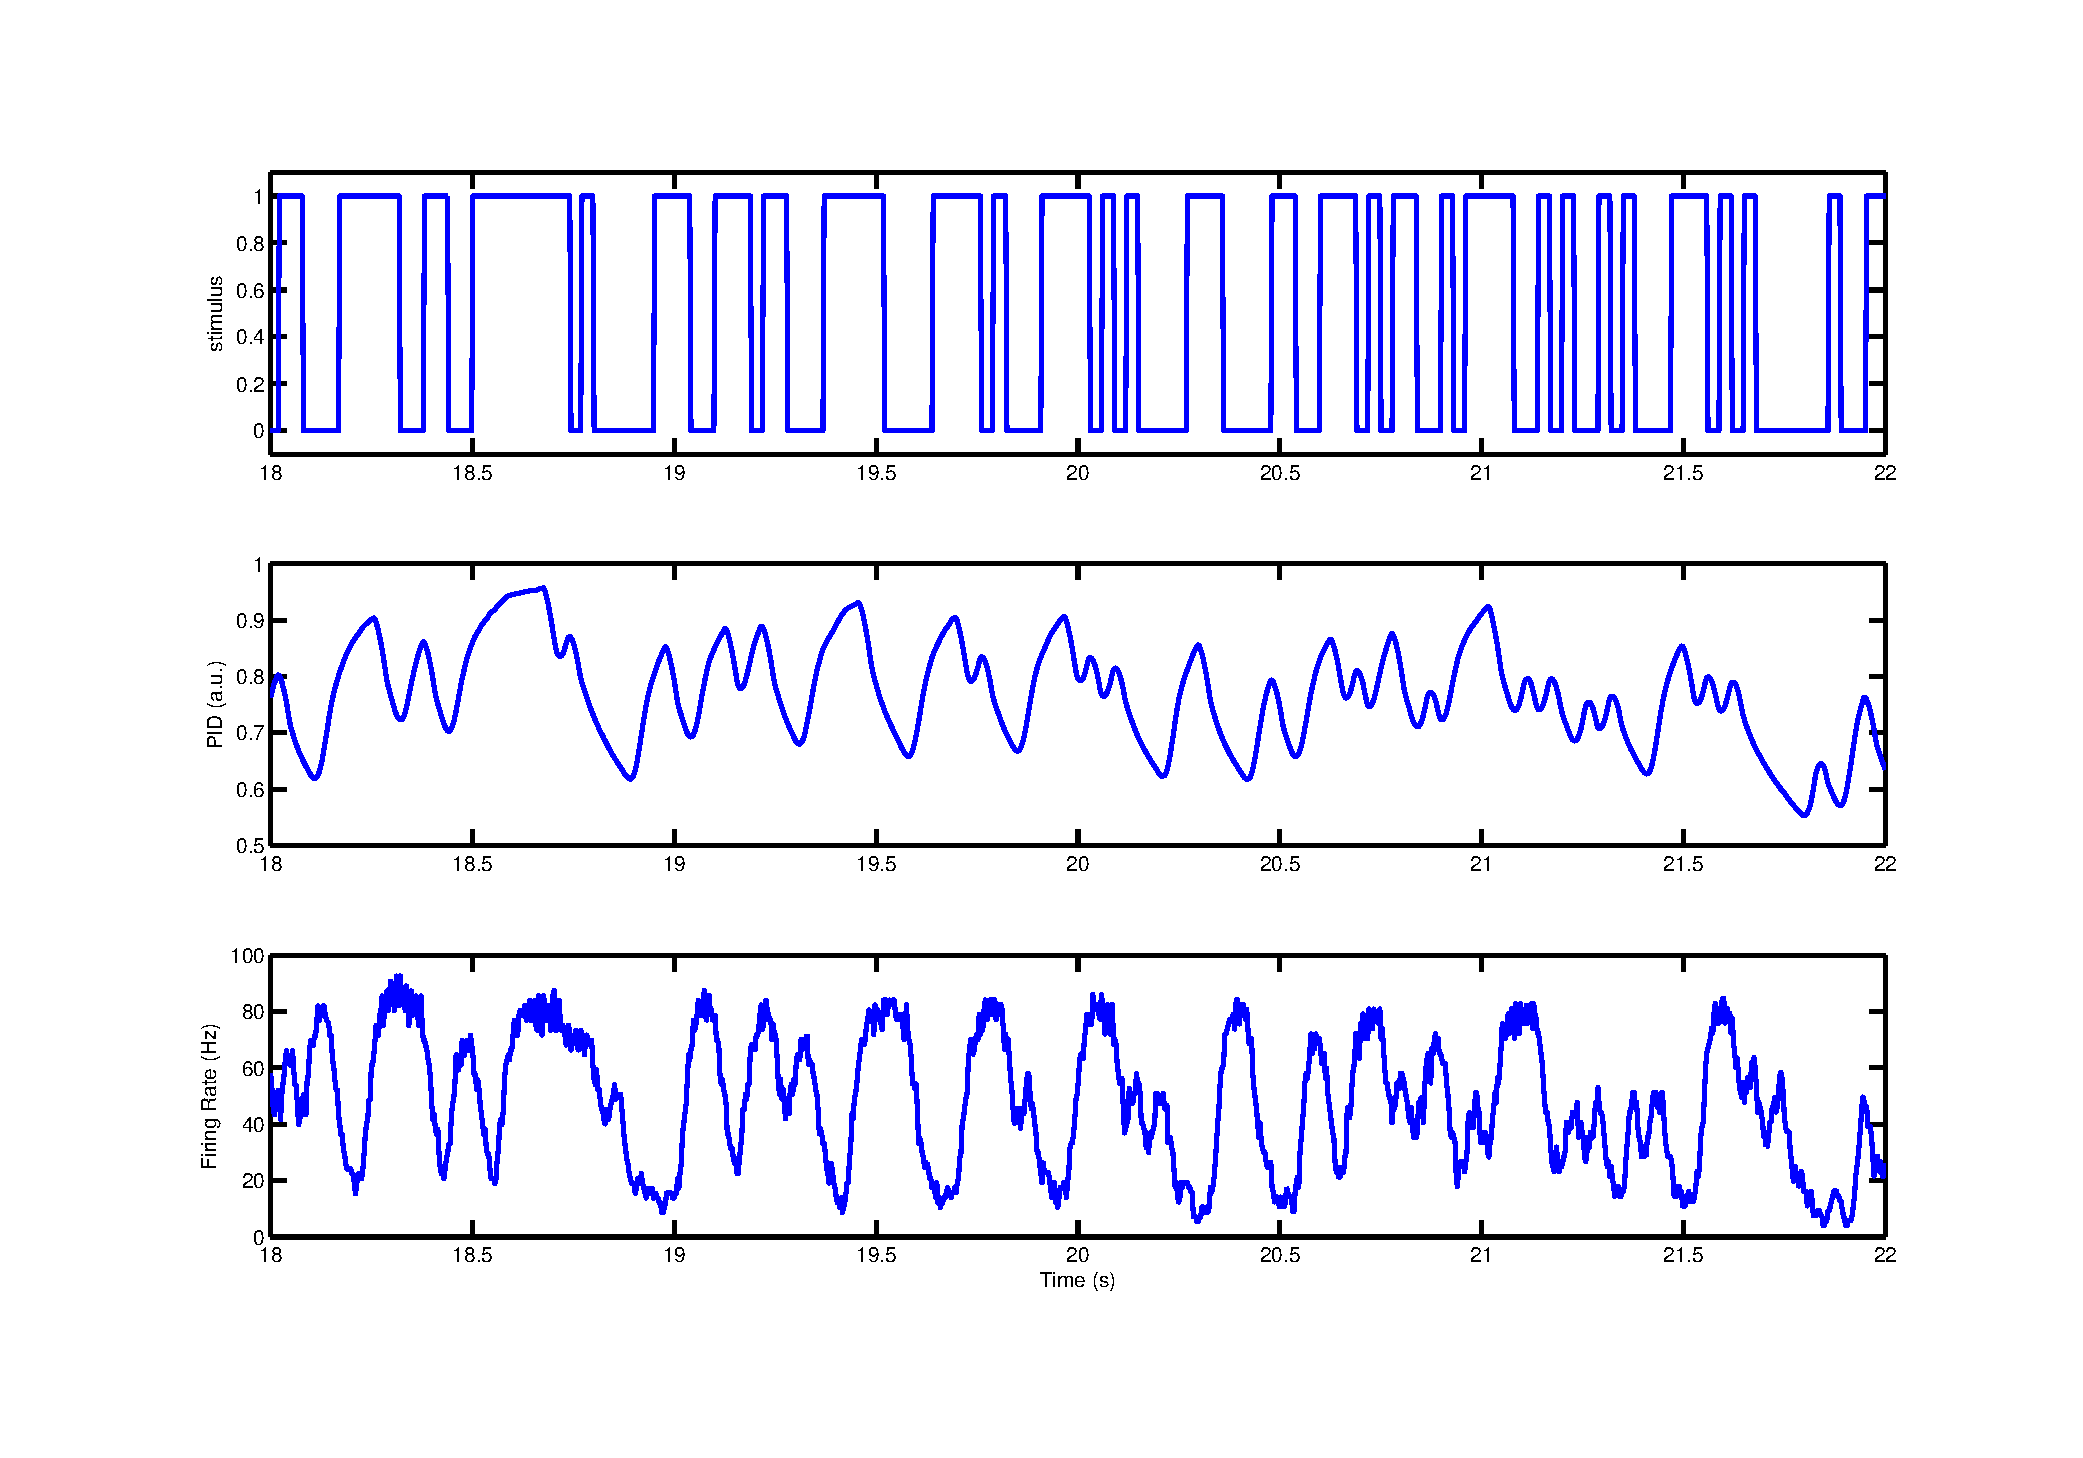
\includegraphics [width=\textwidth]{Analysis_January_01.pdf}
\begin{par}
The odour used, the neuron recorded from and the correlation time of the flickering stimulus are in the file name displayed above the plot.
\end{par} \vspace{1em}


\subsection*{Filter Extraction}

\begin{par}
Details about the filter extraction, regularisation methods, and validation with synthetic and real data is listed in (FilterExtraction.pdf). Here, we calculate the best filter (scaled to ensure that gain = 1) using techniques described in that document from the PID (left) and from the Valve (right).
\end{par} \vspace{1em}

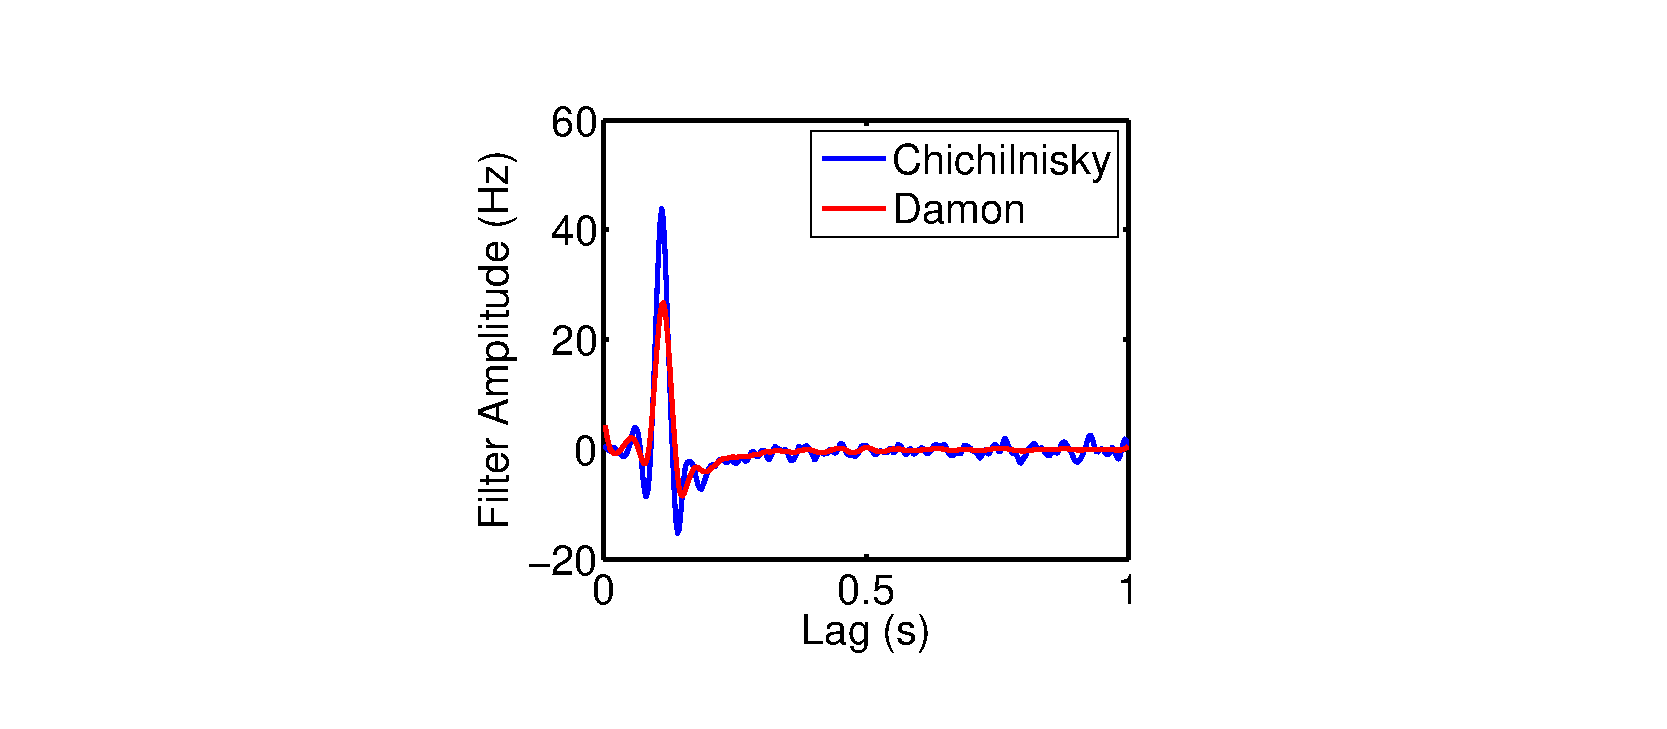
\includegraphics [width=\textwidth]{Analysis_January_02.pdf}
\begin{par}
The variation of filter shape with regularisation parameter for the PID \ensuremath{>} f filter is shown below:
\end{par} \vspace{1em}

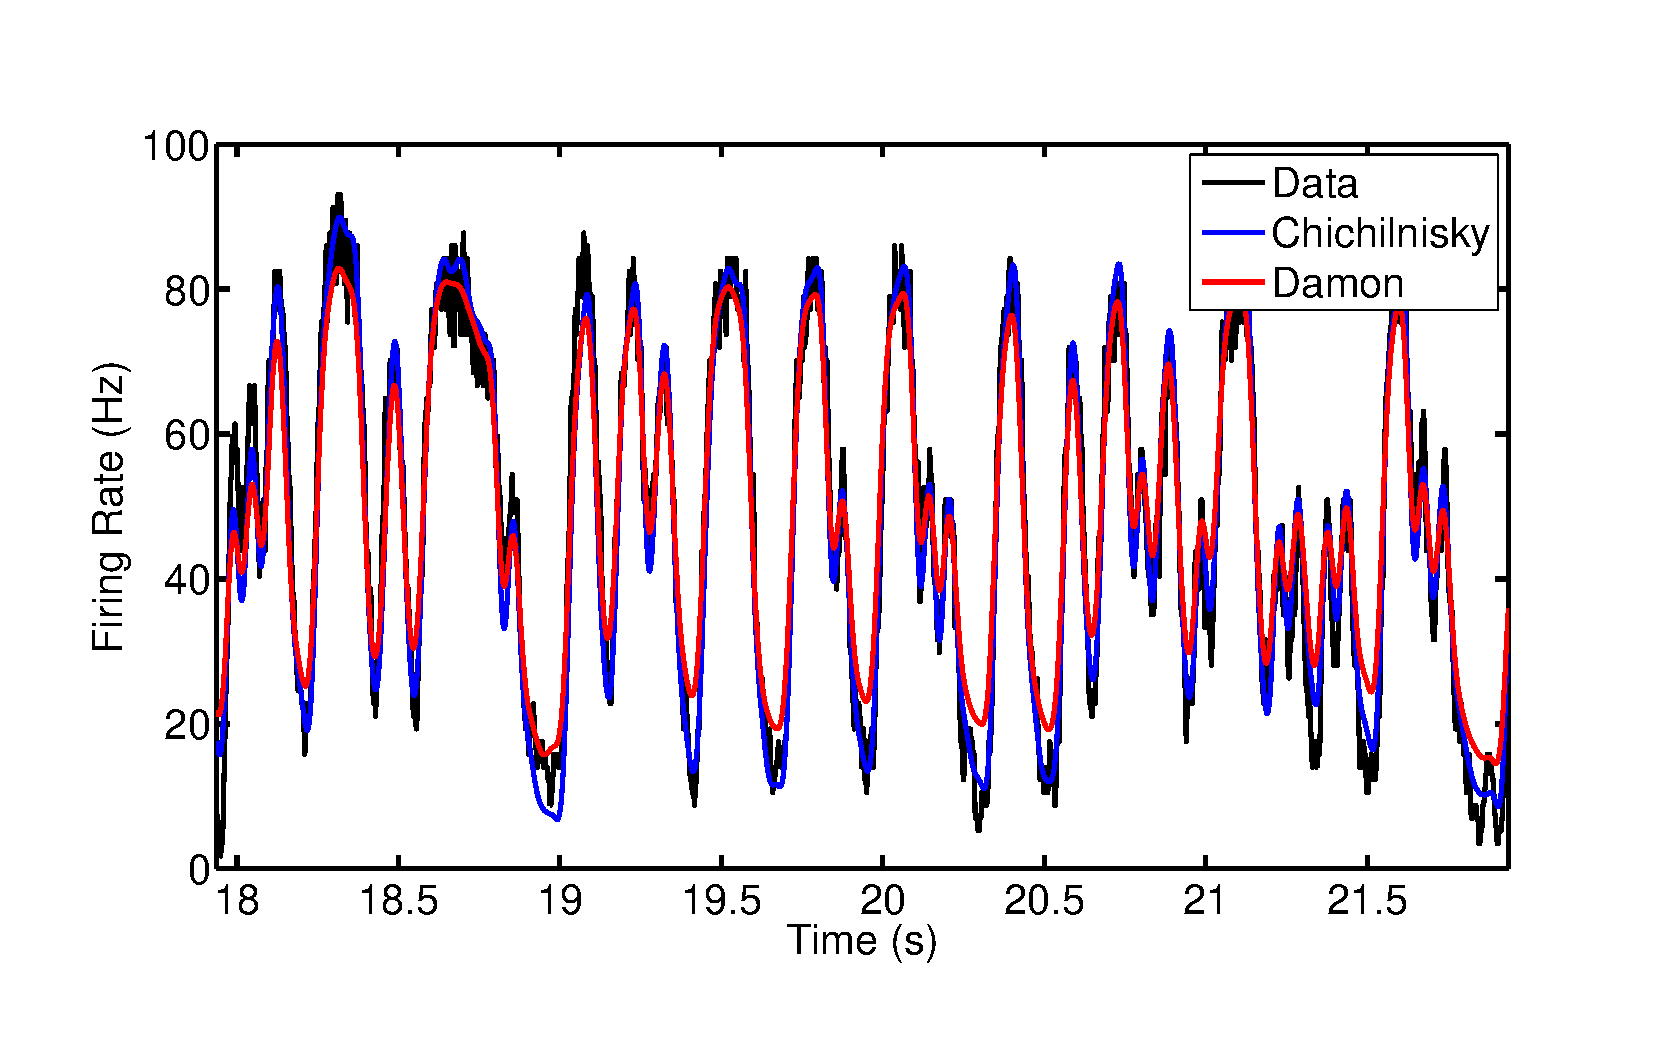
\includegraphics [width=\textwidth]{Analysis_January_03.pdf}
\begin{par}
The variation of filter shape with regularisation parameter for the Valve \ensuremath{>} f filter is shown below:
\end{par} \vspace{1em}

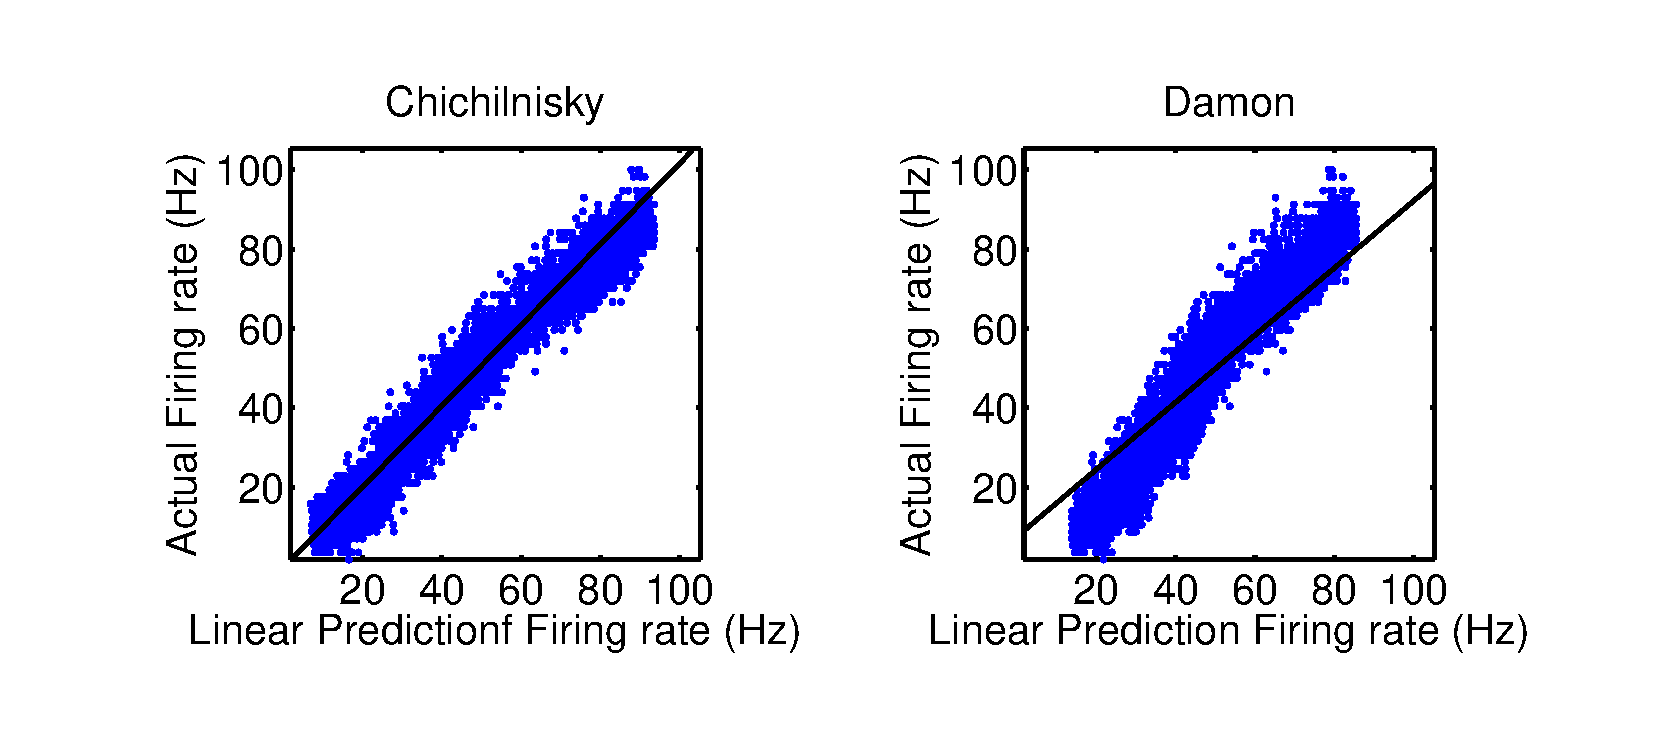
\includegraphics [width=\textwidth]{Analysis_January_04.pdf}
\begin{par}
The convolution of this filter with the input (PID) gives a prediction of the output. In the figure below, the data is shown in black, and the prediction from the PID filter is shown in blue and the prediction from the Valve filter is shown in red. Note that sometimes the prediction can be below zero, which doesn't mean anything physical (firing rate cannot be \ensuremath{<} 0).
\end{par} \vspace{1em}

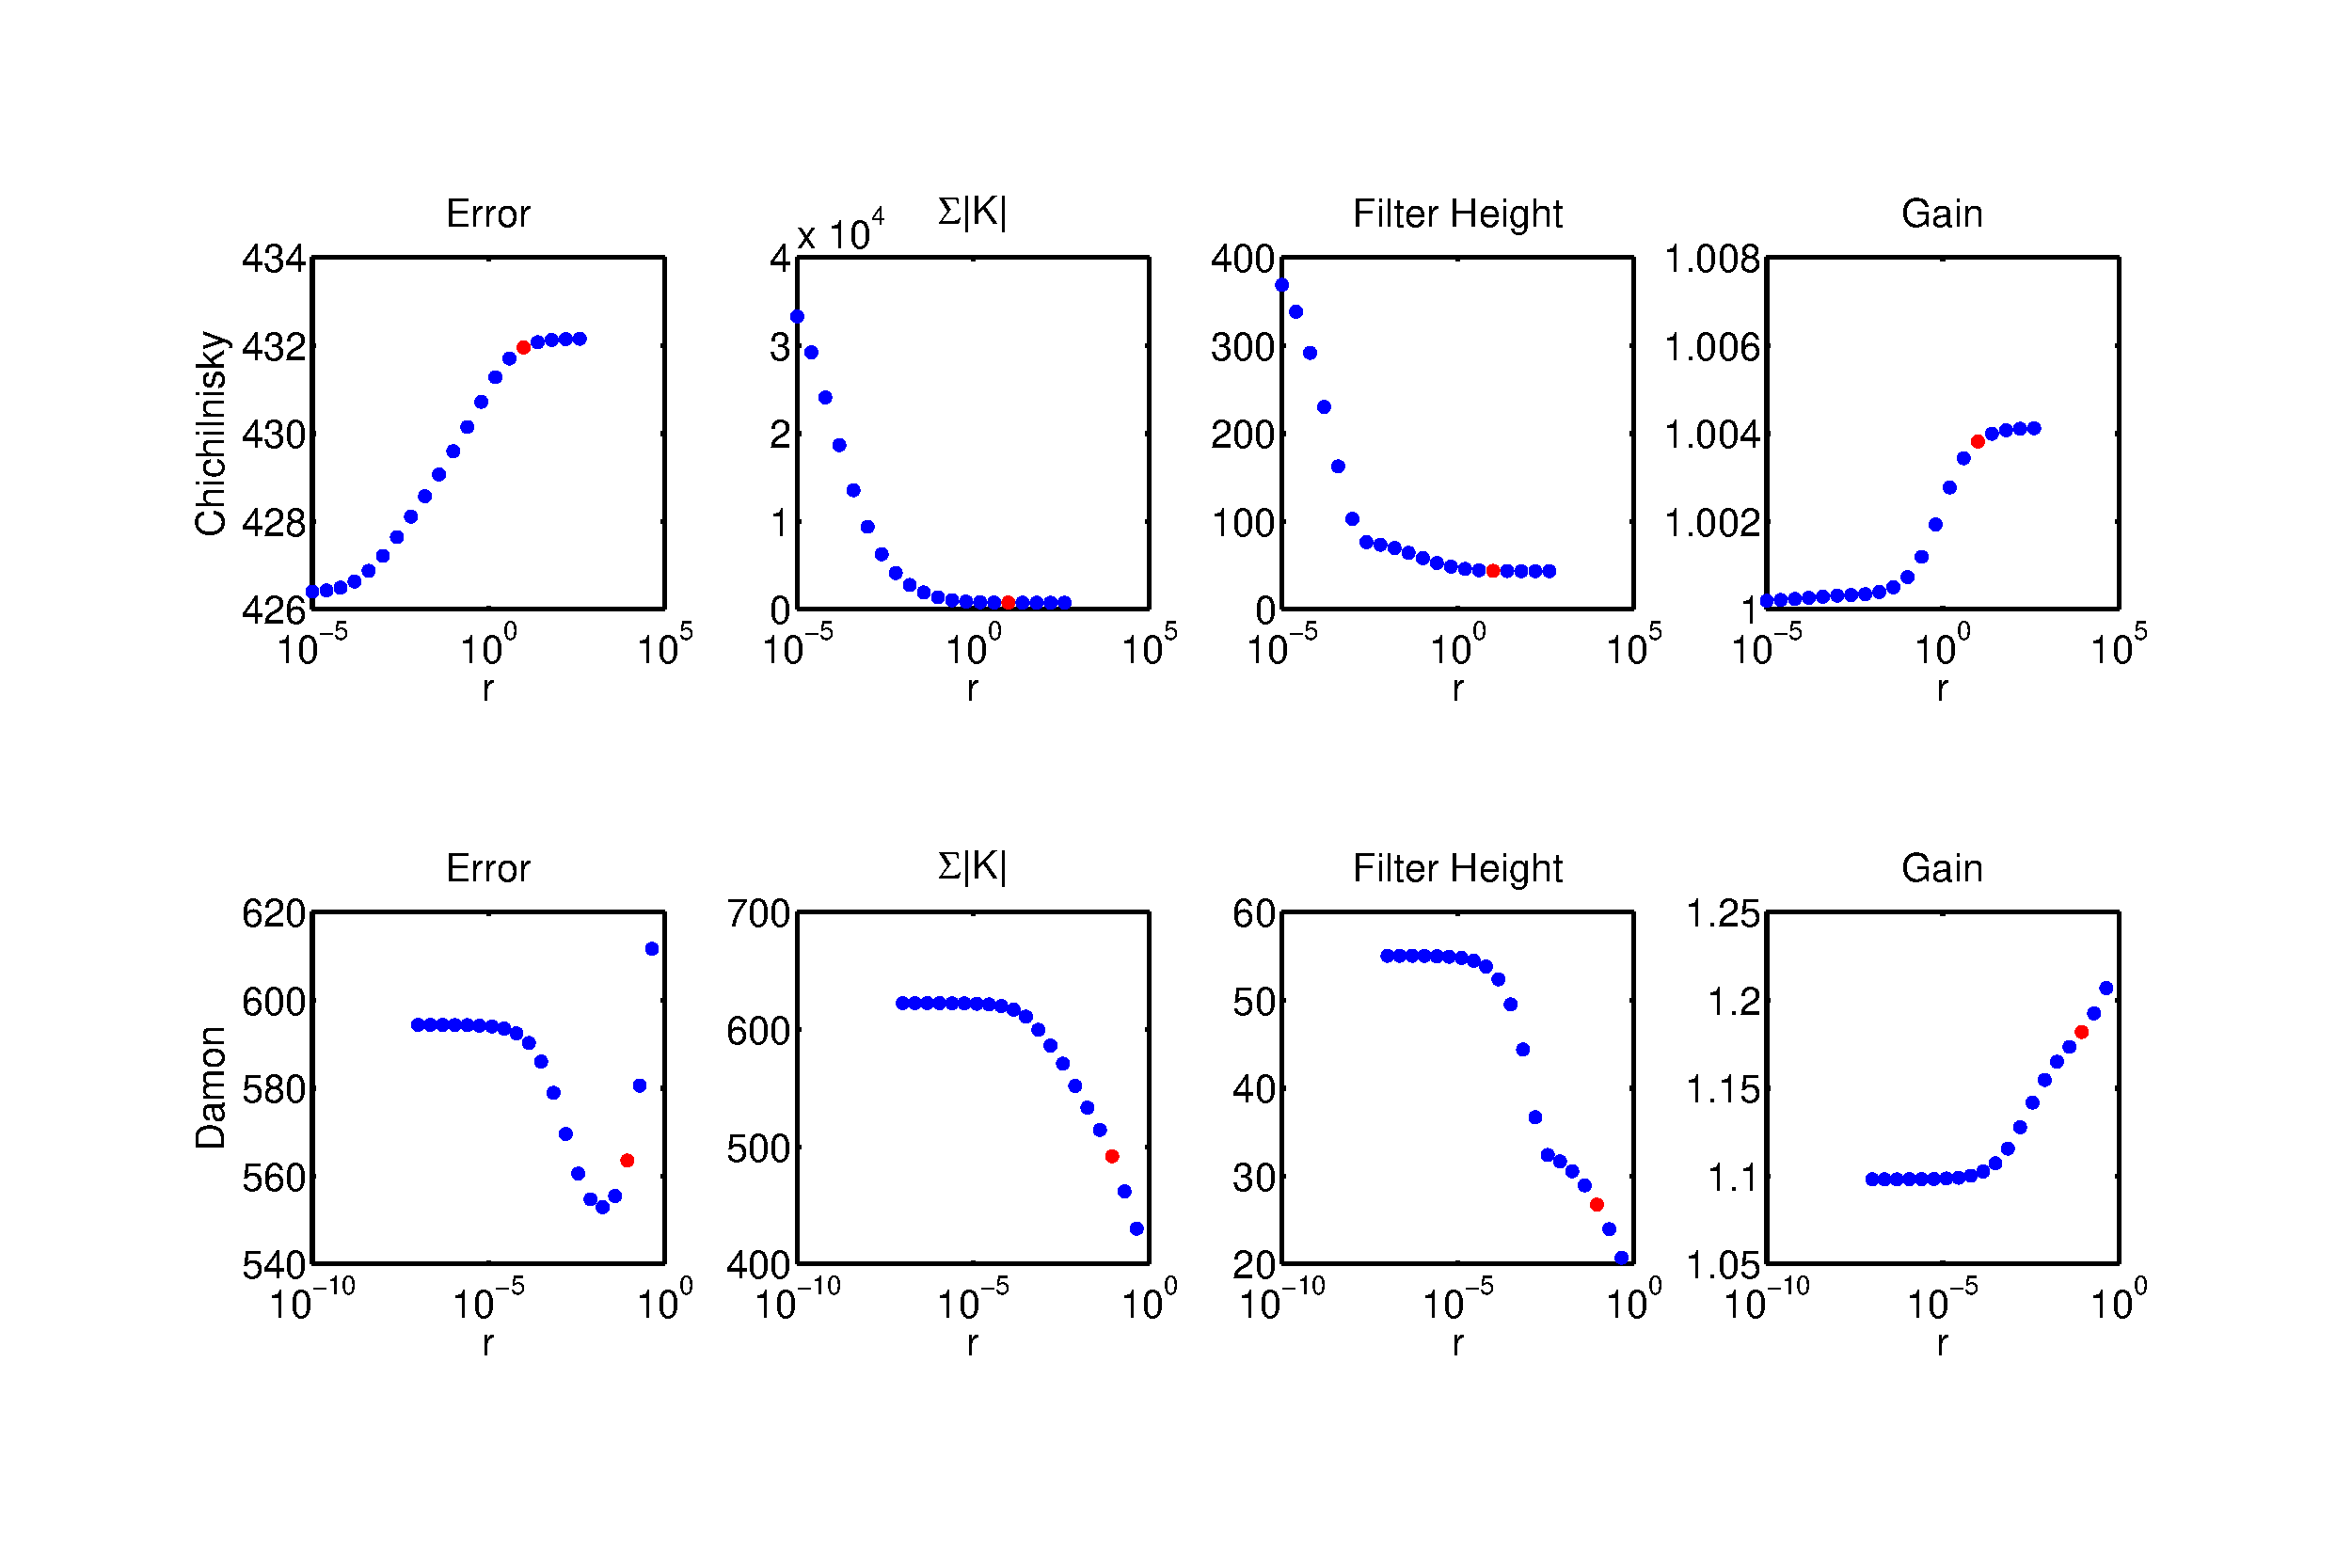
\includegraphics [width=\textwidth]{Analysis_January_05.pdf}


\subsection*{Analysis of Linear Prediction - Which input predicts output better?}

\begin{par}
The measurement of the stimulus should help us predict the response of the neuron better than just the valve control signal, as we now capture the fast fluctuations of the odour stimulus as it reaches the ORN. Thus, a prediction of ORN firing response from the PID signal should be better than a prediction of the ORN firing response from the valve signal.
\end{par} \vspace{1em}
\begin{par}
The r-square (coefficient of determination) of the PID\ensuremath{>}f prediction is:
\end{par} \vspace{1em}

        \color{lightgray} \begin{verbatim}    0.9276

\end{verbatim} \color{black}
    \begin{par}
The r-square (coefficient of determination) of the Valve\ensuremath{>}f prediction is:
\end{par} \vspace{1em}

        \color{lightgray} \begin{verbatim}    0.9460

\end{verbatim} \color{black}
    

\subsection*{Analysis of Linear Prediction - Linearity of Prediction}

\begin{par}
For a linear filter calculated from the data, a plot of the actual response to the predicted response can be fit with a line of slope 1. Here the actual firing rate is plotted on the X axis and the firing rate predicted from the linear filter is plotted on the Y axis.
\end{par} \vspace{1em}

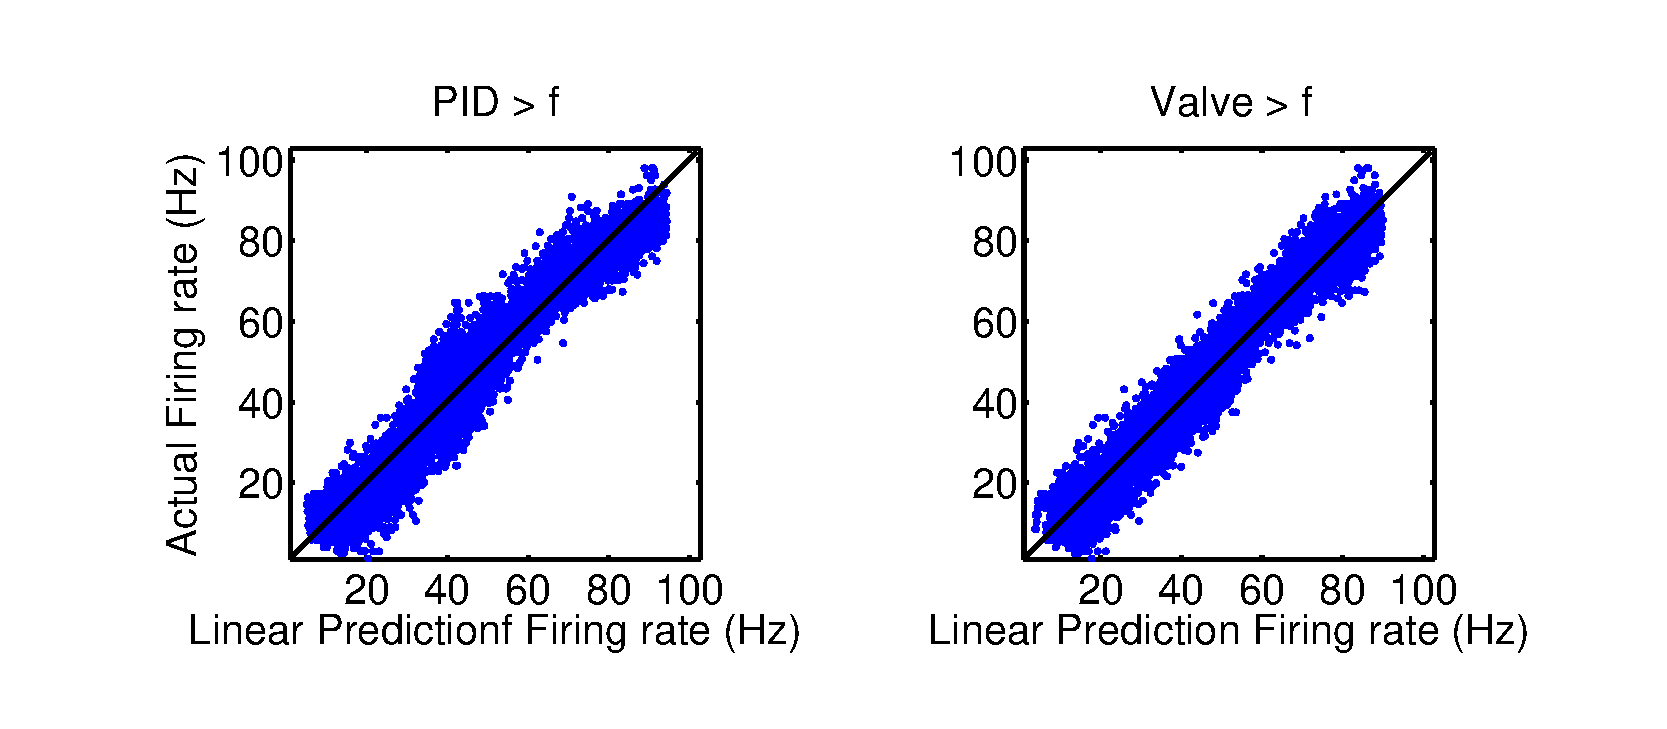
\includegraphics [width=\textwidth]{Analysis_January_06.pdf}
\begin{par}
The line is a best fit to all the data. The slope of the best fit line for the prediction from PID is:
\end{par} \vspace{1em}

        \color{lightgray} \begin{verbatim}    1.0000

\end{verbatim} \color{black}
    \begin{par}
The line is a best fit to all the data. The slope of the best fit line for the prediction from the valve is:
\end{par} \vspace{1em}

        \color{lightgray} \begin{verbatim}    1.0000

\end{verbatim} \color{black}
    

\subsection*{Analysis of Linear Prediction - Response to High and Low Stimuli}

\begin{par}
How does the response of the ORN differ for high and low stimuli? Specifically, does the neuron display the characteristics of fast adaptation to this flickering stimulus?
\end{par} \vspace{1em}
\begin{par}
To look at this, we calculate the mean average stimulus over some window history length for every time point \textit{t}, for various different window history lengths. The effect of this operation is shown in the figure below, where the legend refers to the history window in ms.
\end{par} \vspace{1em}

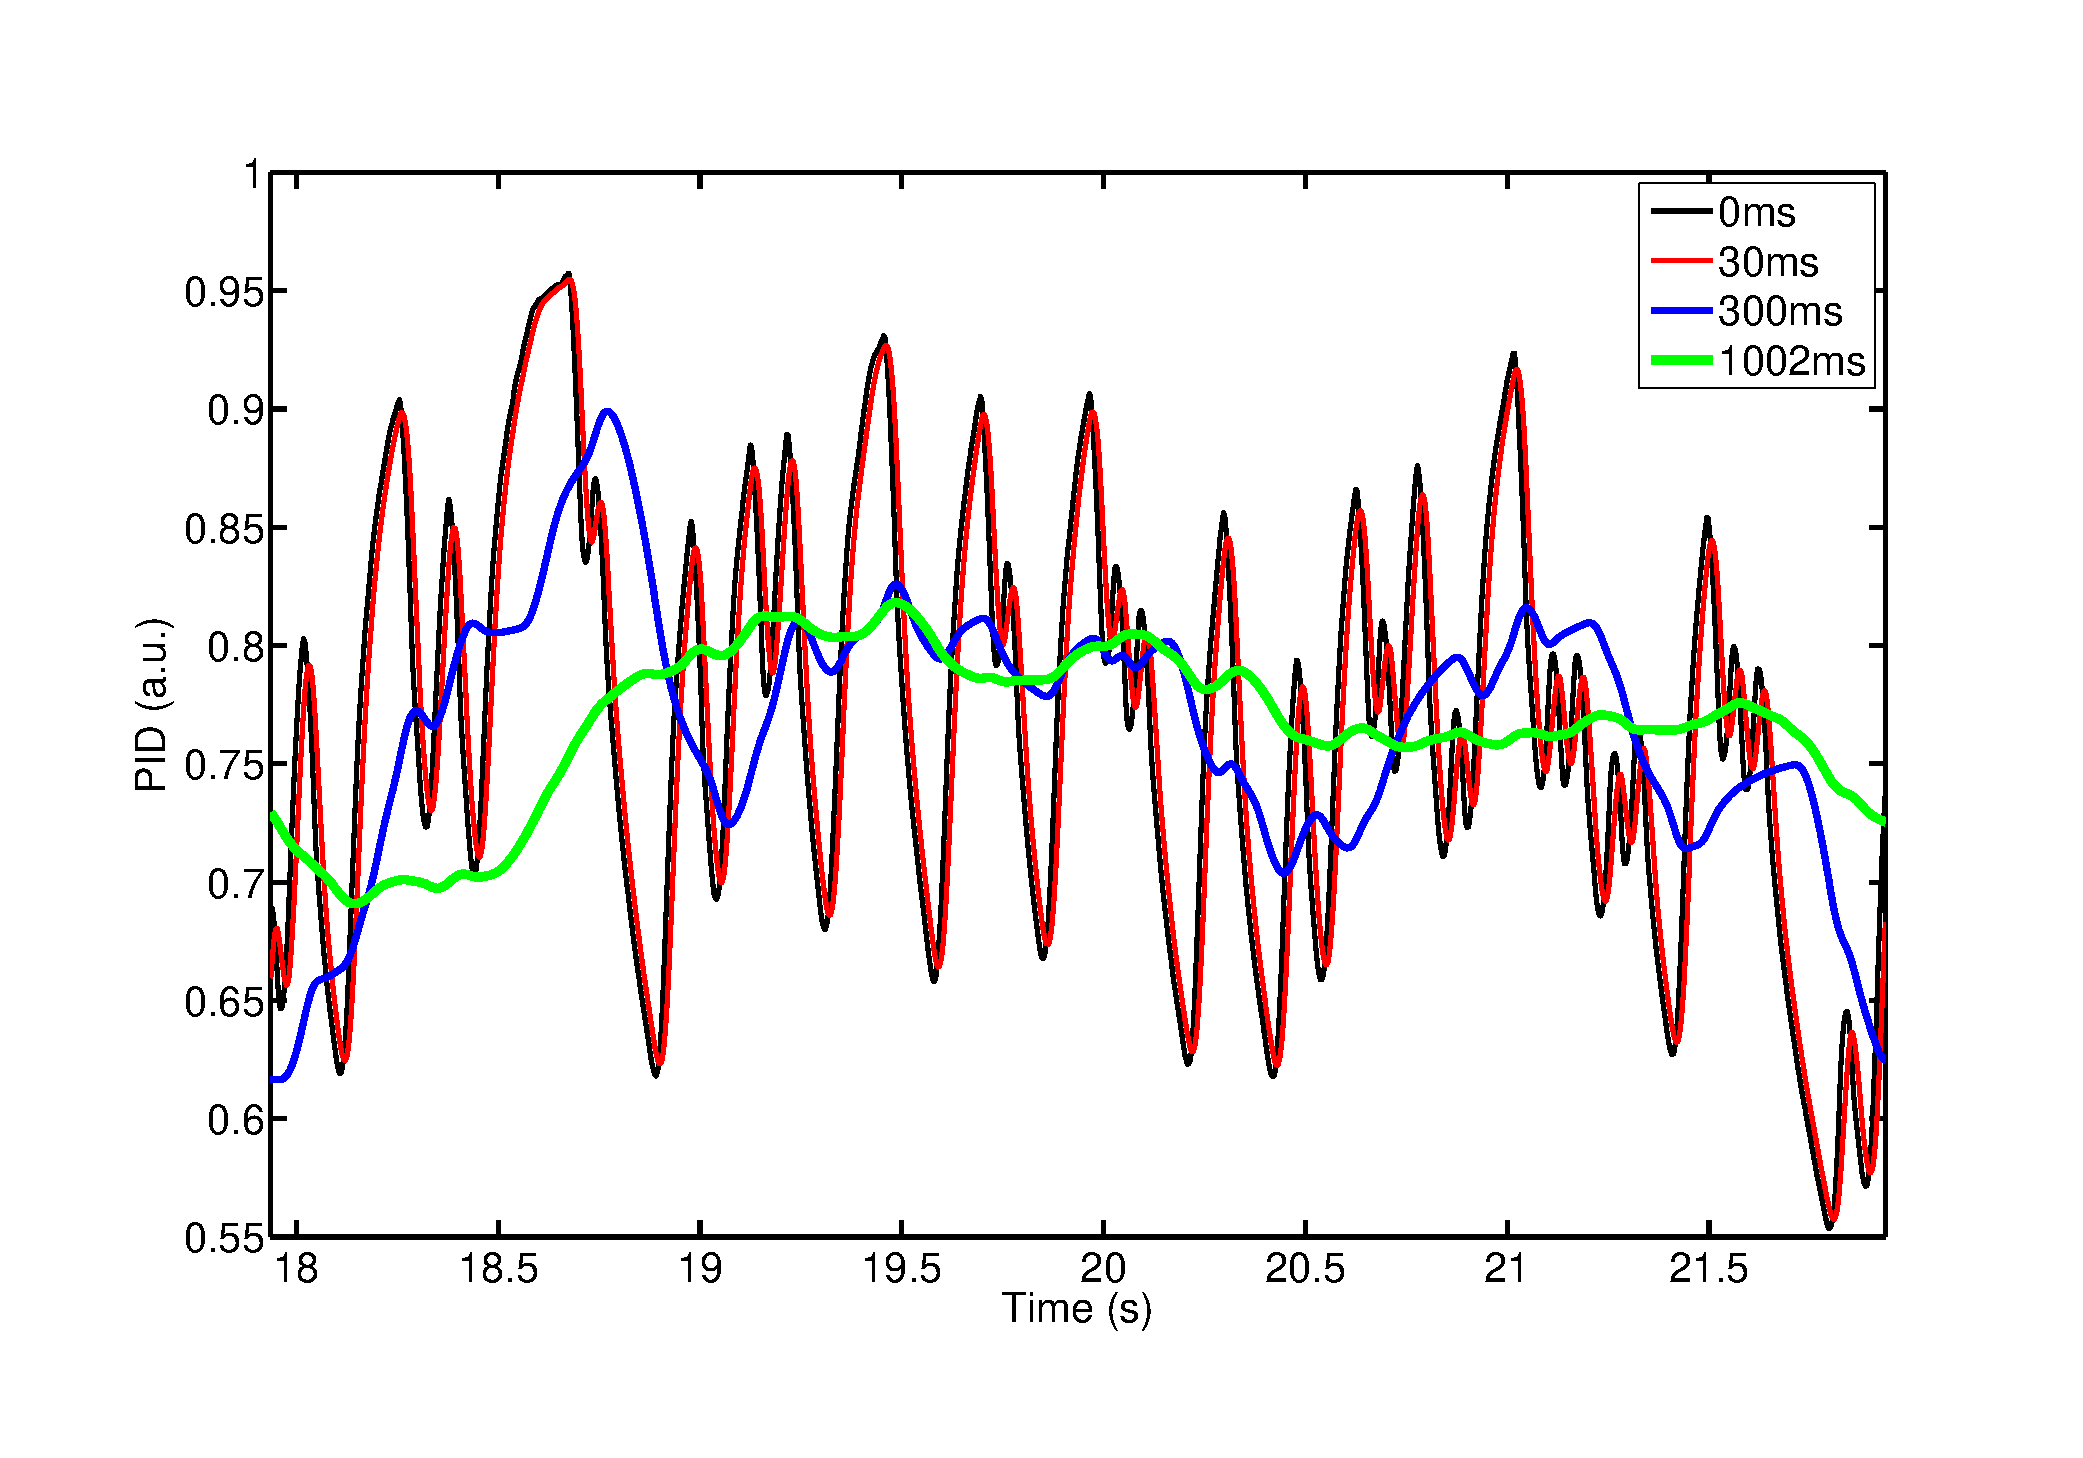
\includegraphics [width=\textwidth]{Analysis_January_07.pdf}
\begin{par}
Now, we separate neuron responses and linear prediction at times when the mean average stimulus is in the lowest 10\% or the highest 10\%. These points are marked either green (lowest 10\%) or red (or highest 10\%) in the figures below, while all the data is plotted in grey. Lines are fit to each of these clouds of points, and the slopes (representing the instantaneous gain) is calculated from these lines. The \textit{y} axis is the actual firing rate, while the \textit{x} axis is the predicted firing rate. In this analysis the prediction from the PID is used.
\end{par} \vspace{1em}

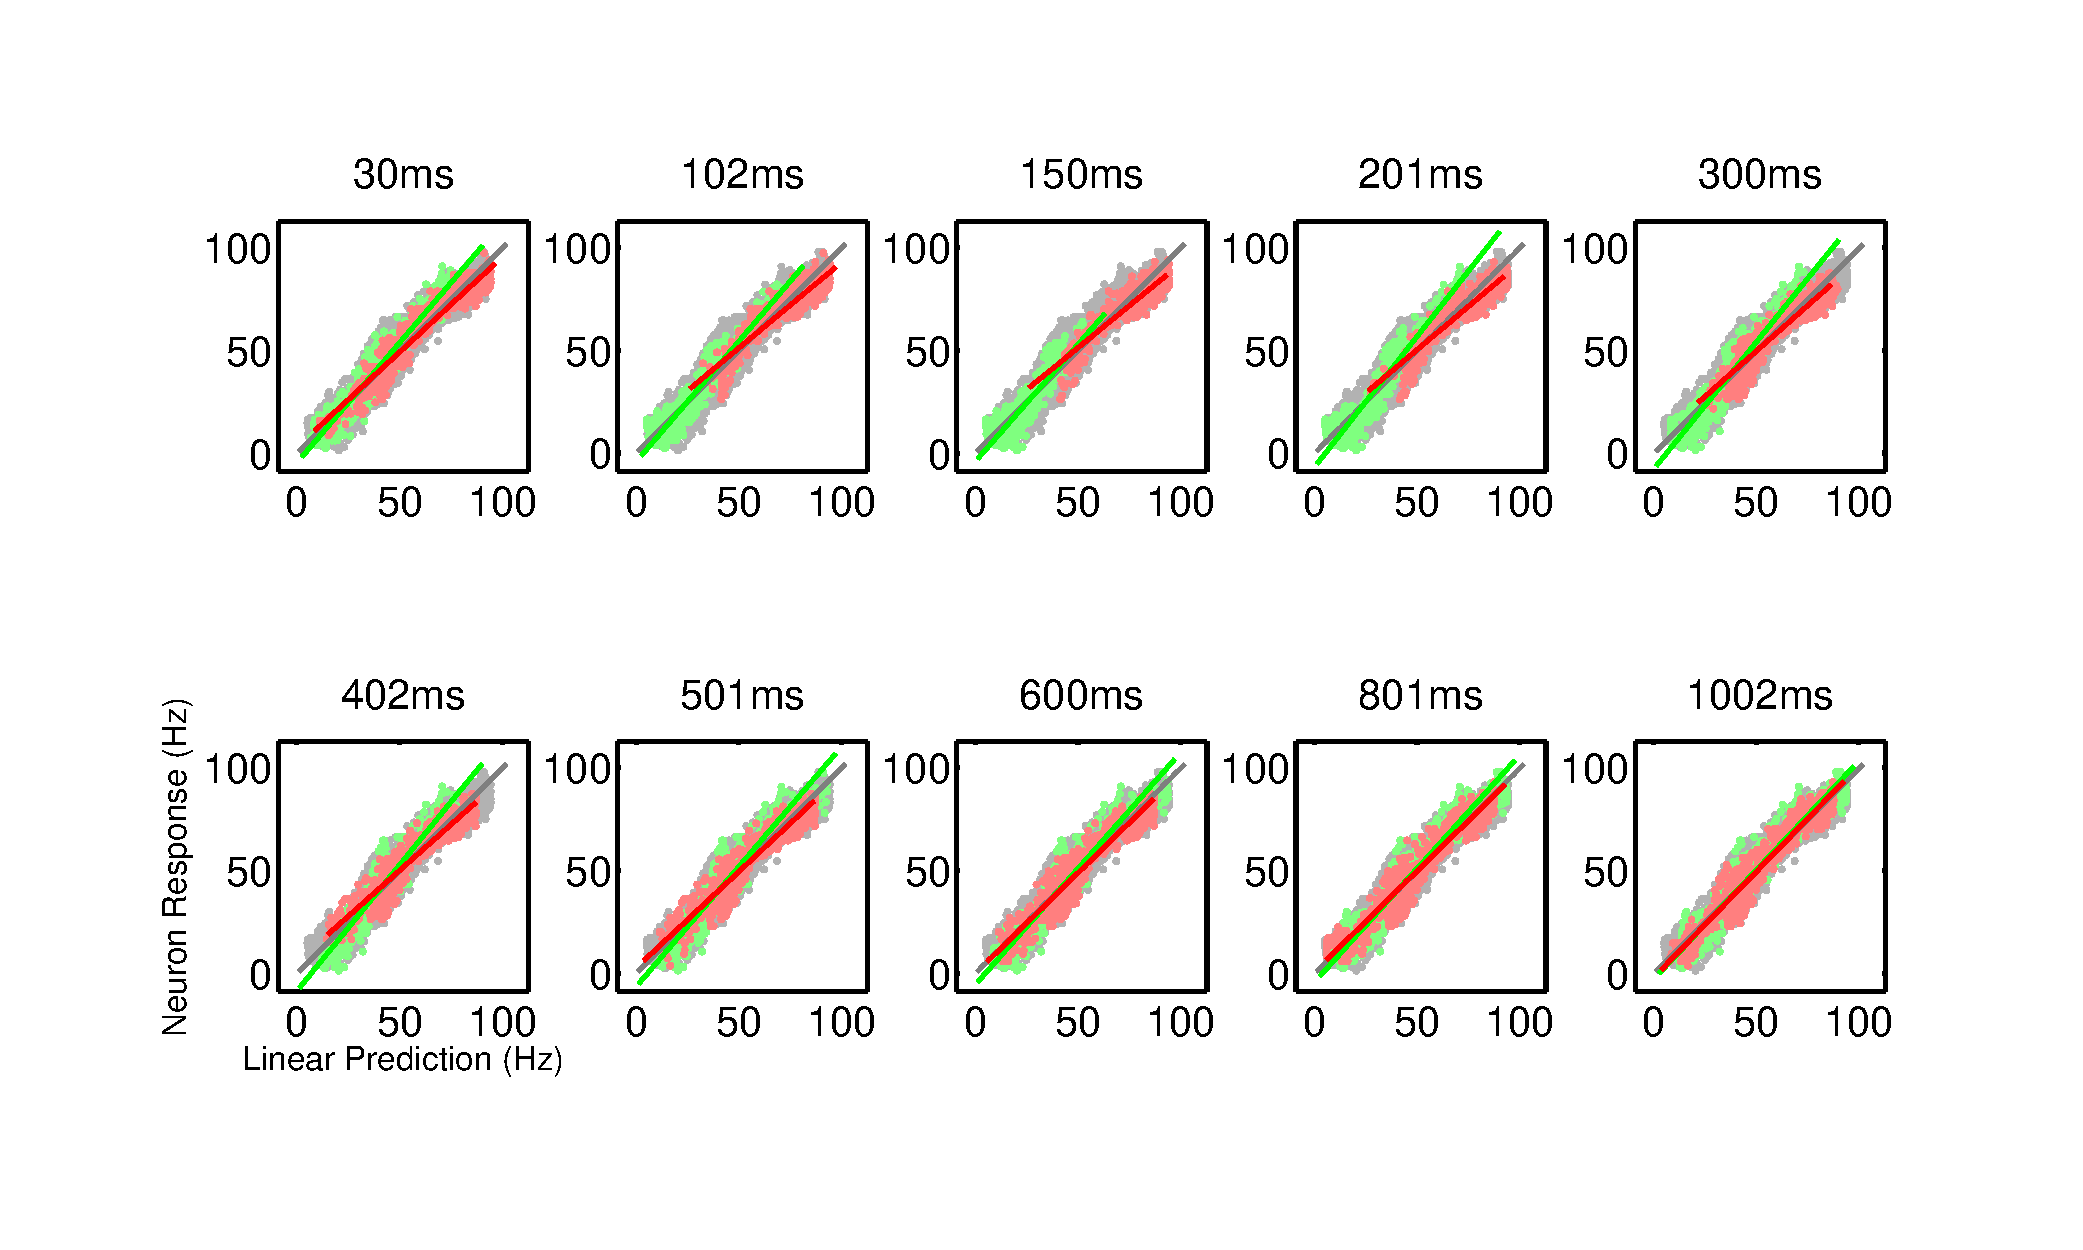
\includegraphics [width=\textwidth]{Analysis_January_08.pdf}
\begin{par}
The following plot shows how the slope of the lines of best fit, or the instantaneous gains, varies with the history length. The plot on the right shows the goodness of fit for each fit, indicating the regions where the fit is meaningful.
\end{par} \vspace{1em}

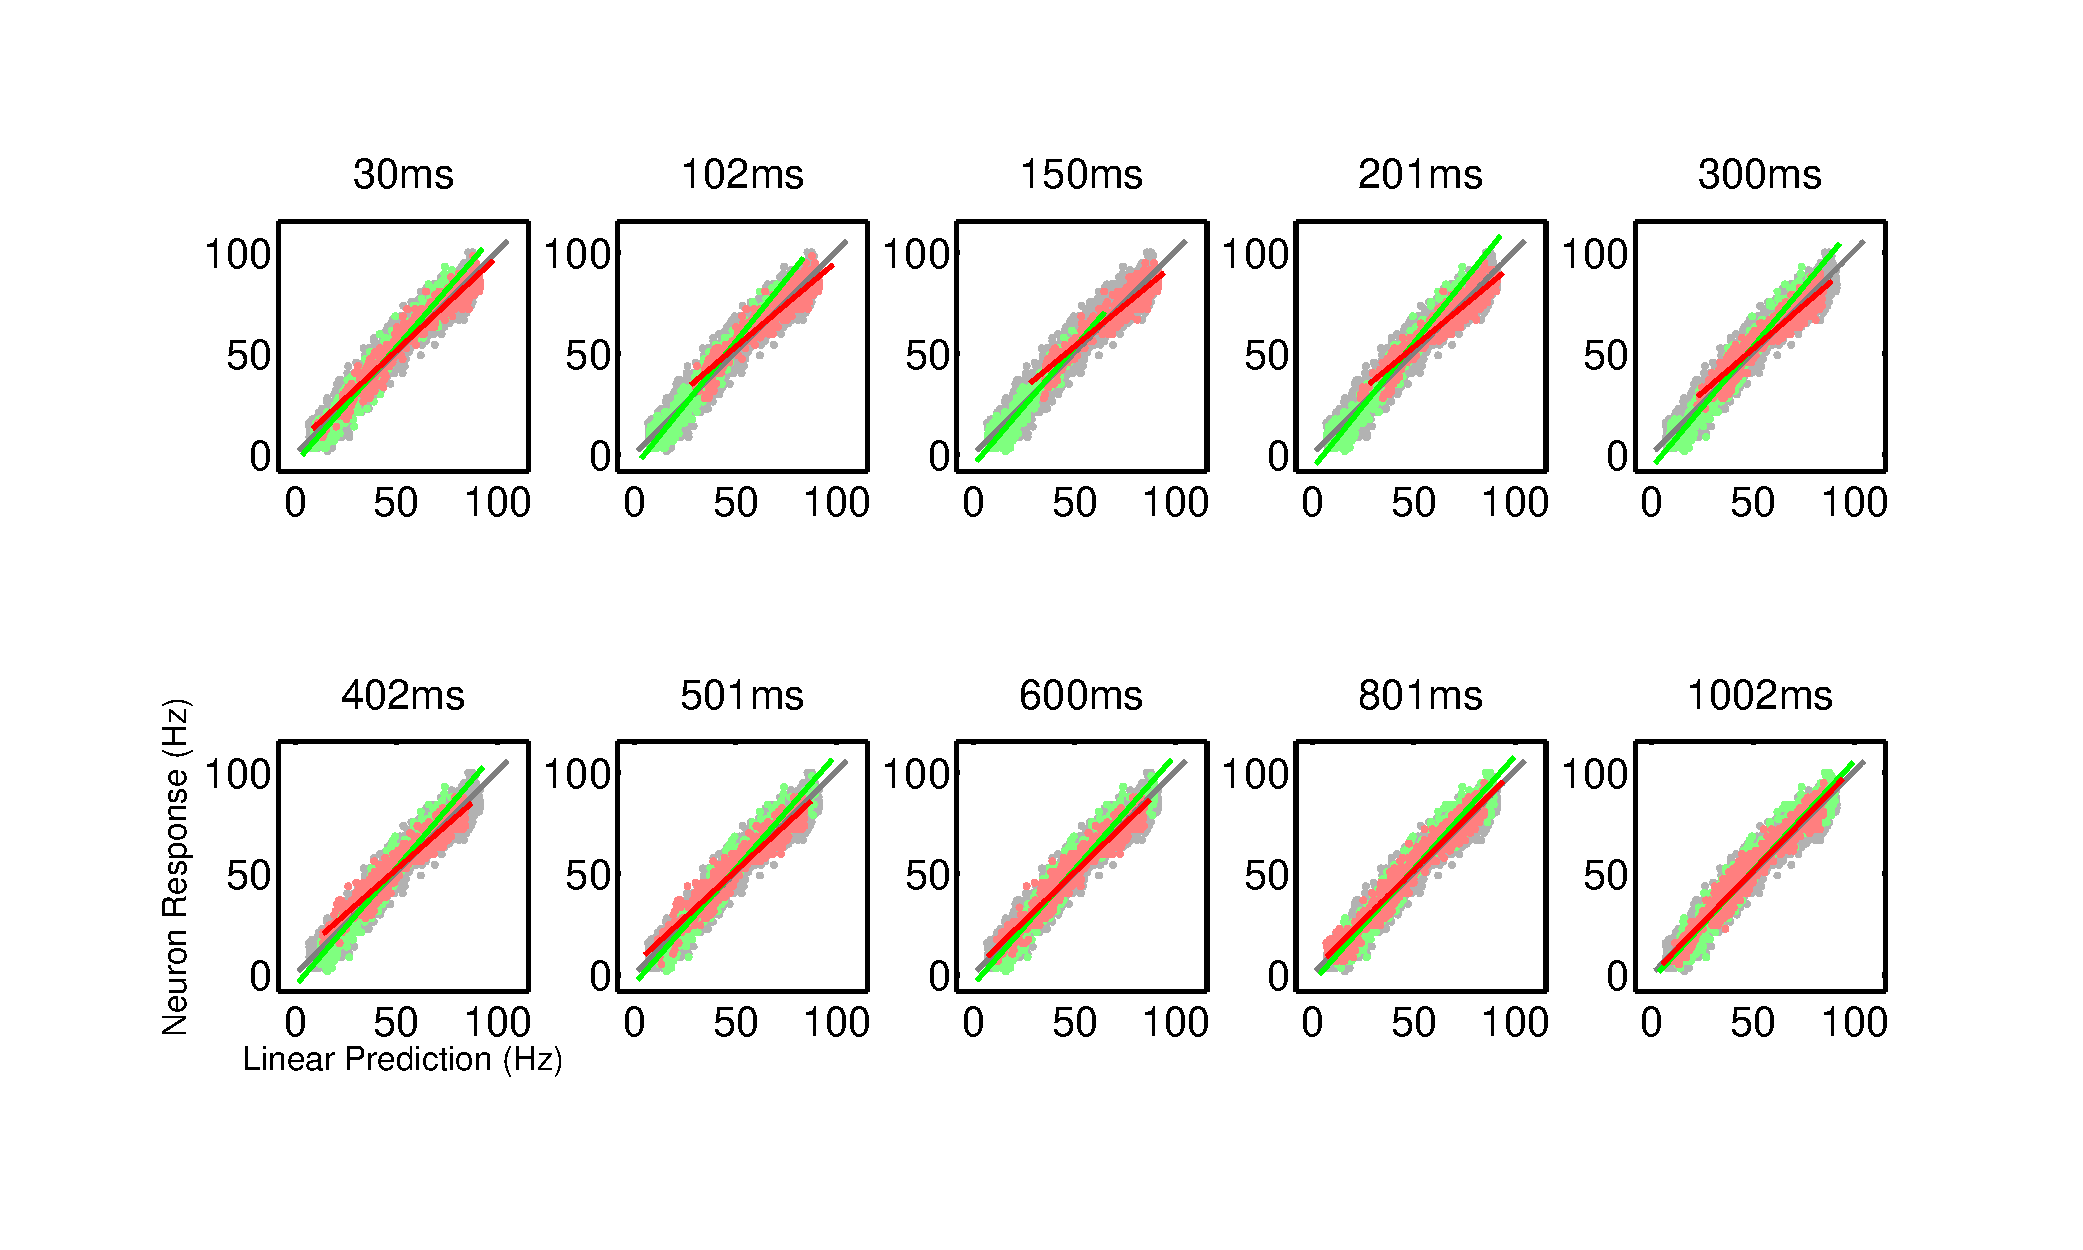
\includegraphics [width=\textwidth]{Analysis_January_09.pdf}


\subsection*{Analysis of Linear Prediction - Filter Variation (to be done)}

\begin{par}
We have segmented the entire data set based on when the stimulus, averaged in some way over the past, into high and low. Here, I will calculate filters for each of these subsets.
\end{par} \vspace{1em}


\subsection*{Analysis of Linear Prediction - Does adding another linear filter improve prediction?}

\begin{par}
An ideal linear filter should capture all the linear variation in the data. This means that if one were to construct a vector of residuals, a linear filter would be unable to predict the residuals from the data, and would lead to no improvement on the original filter. Is this true?
\end{par} \vspace{1em}
\begin{par}
First, we construct a vector of residuals by subtracting the linear prediction from the data.
\end{par} \vspace{1em}

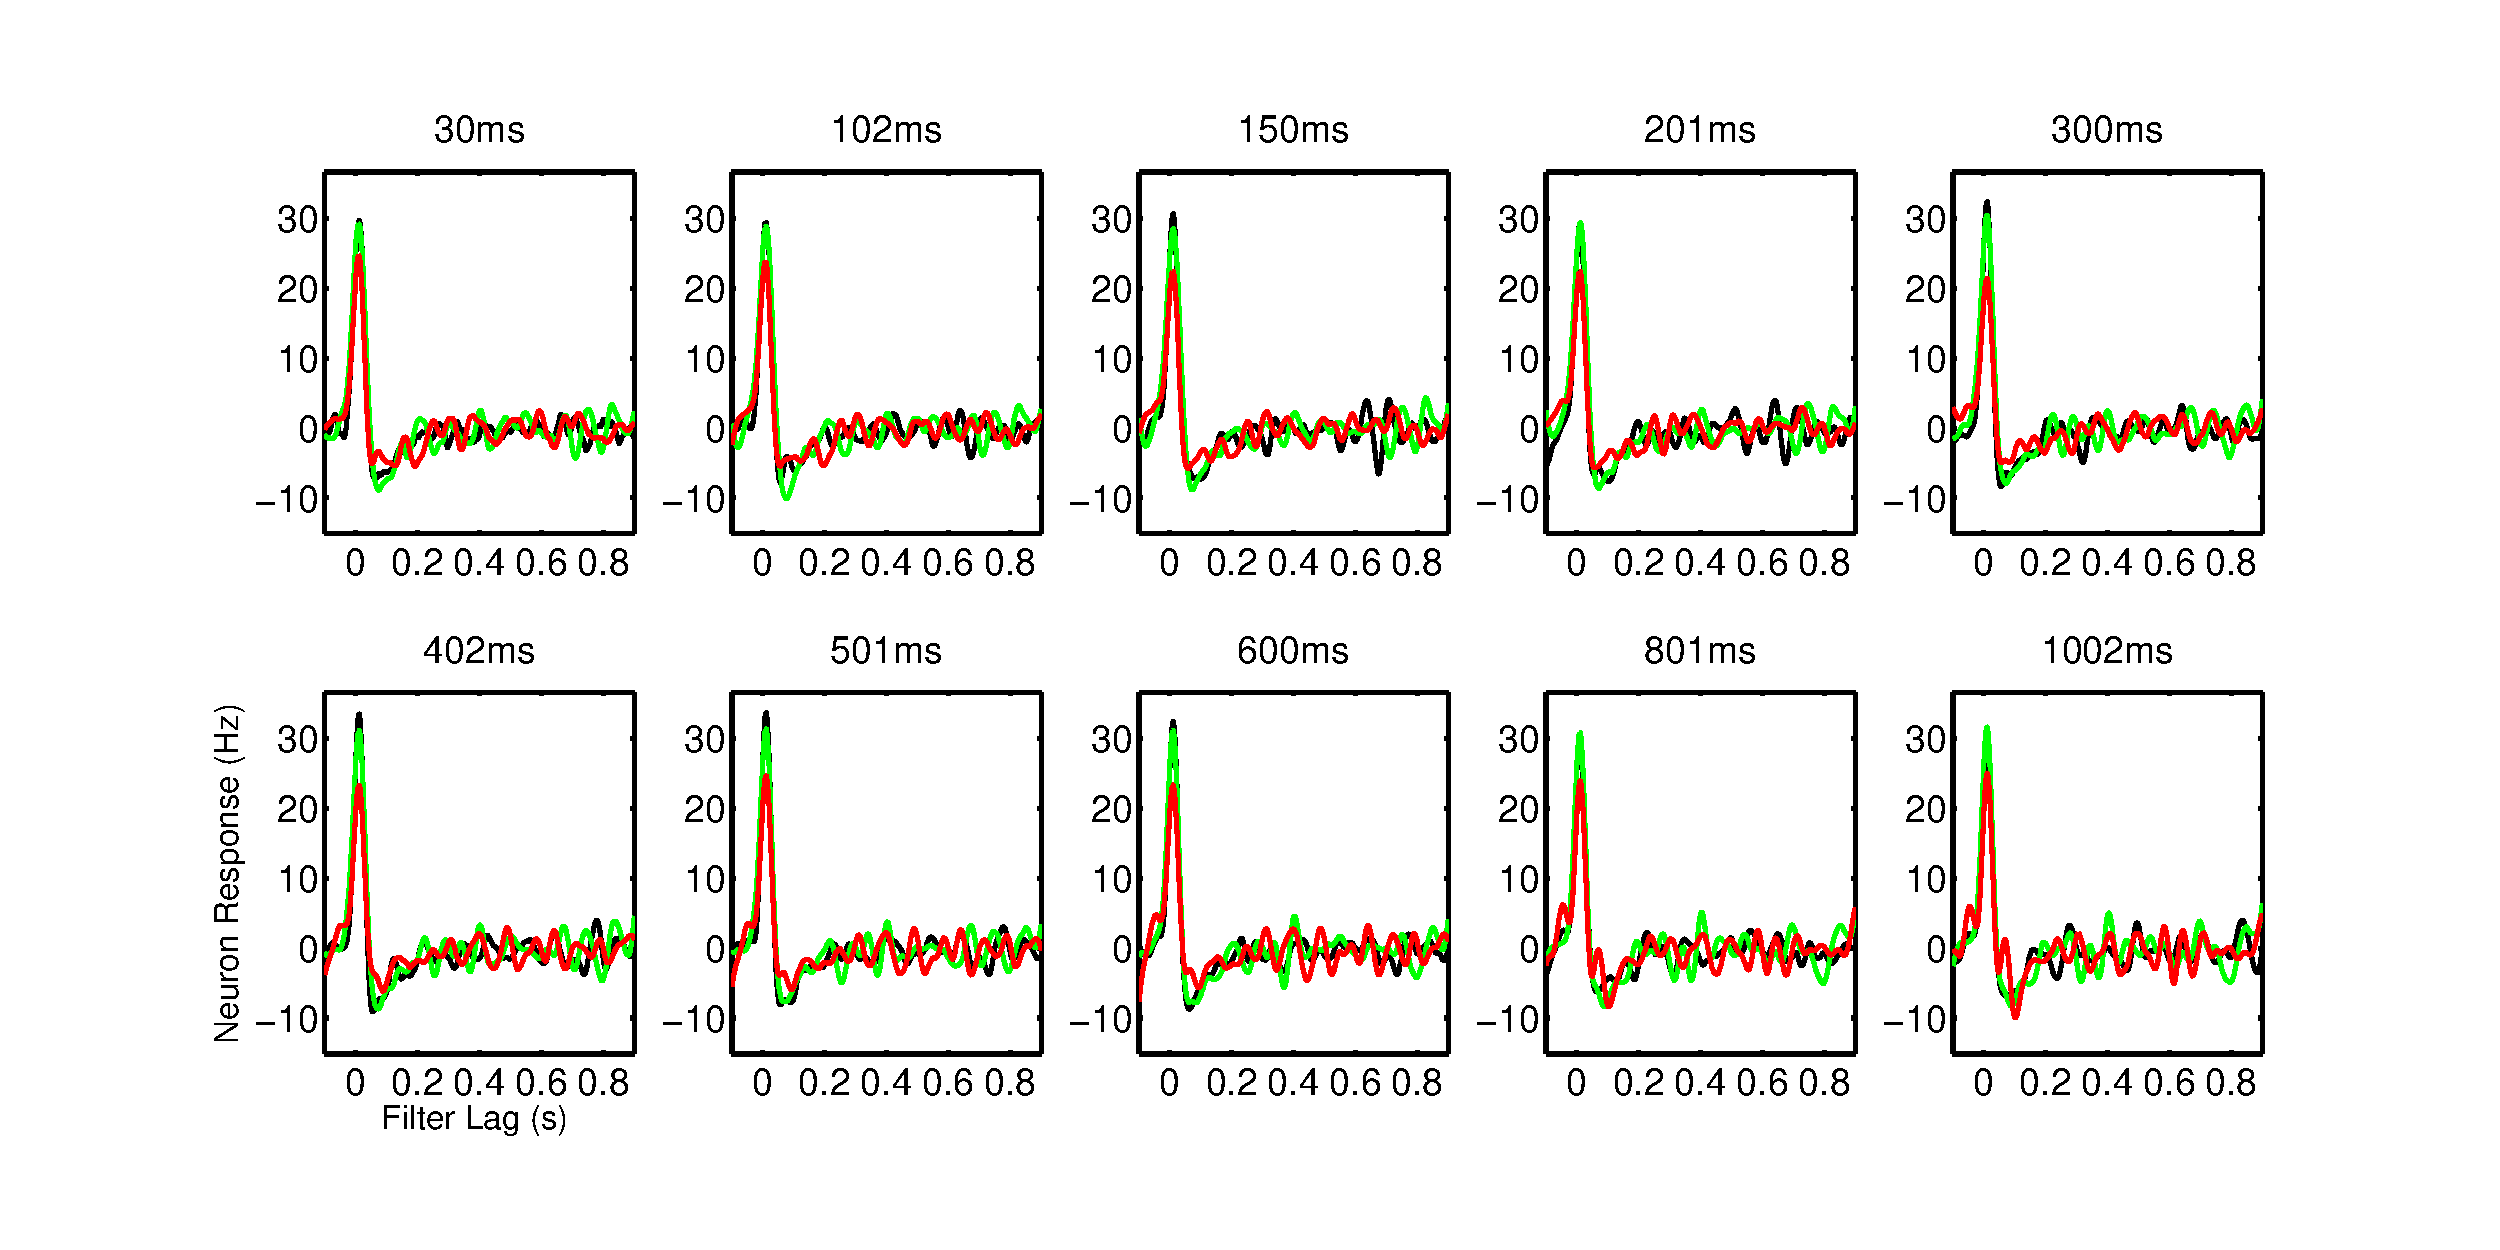
\includegraphics [width=\textwidth]{Analysis_January_10.pdf}
\begin{par}
we then construct a filter from the PID to these residuals to try to predict the residuals.
\end{par} \vspace{1em}

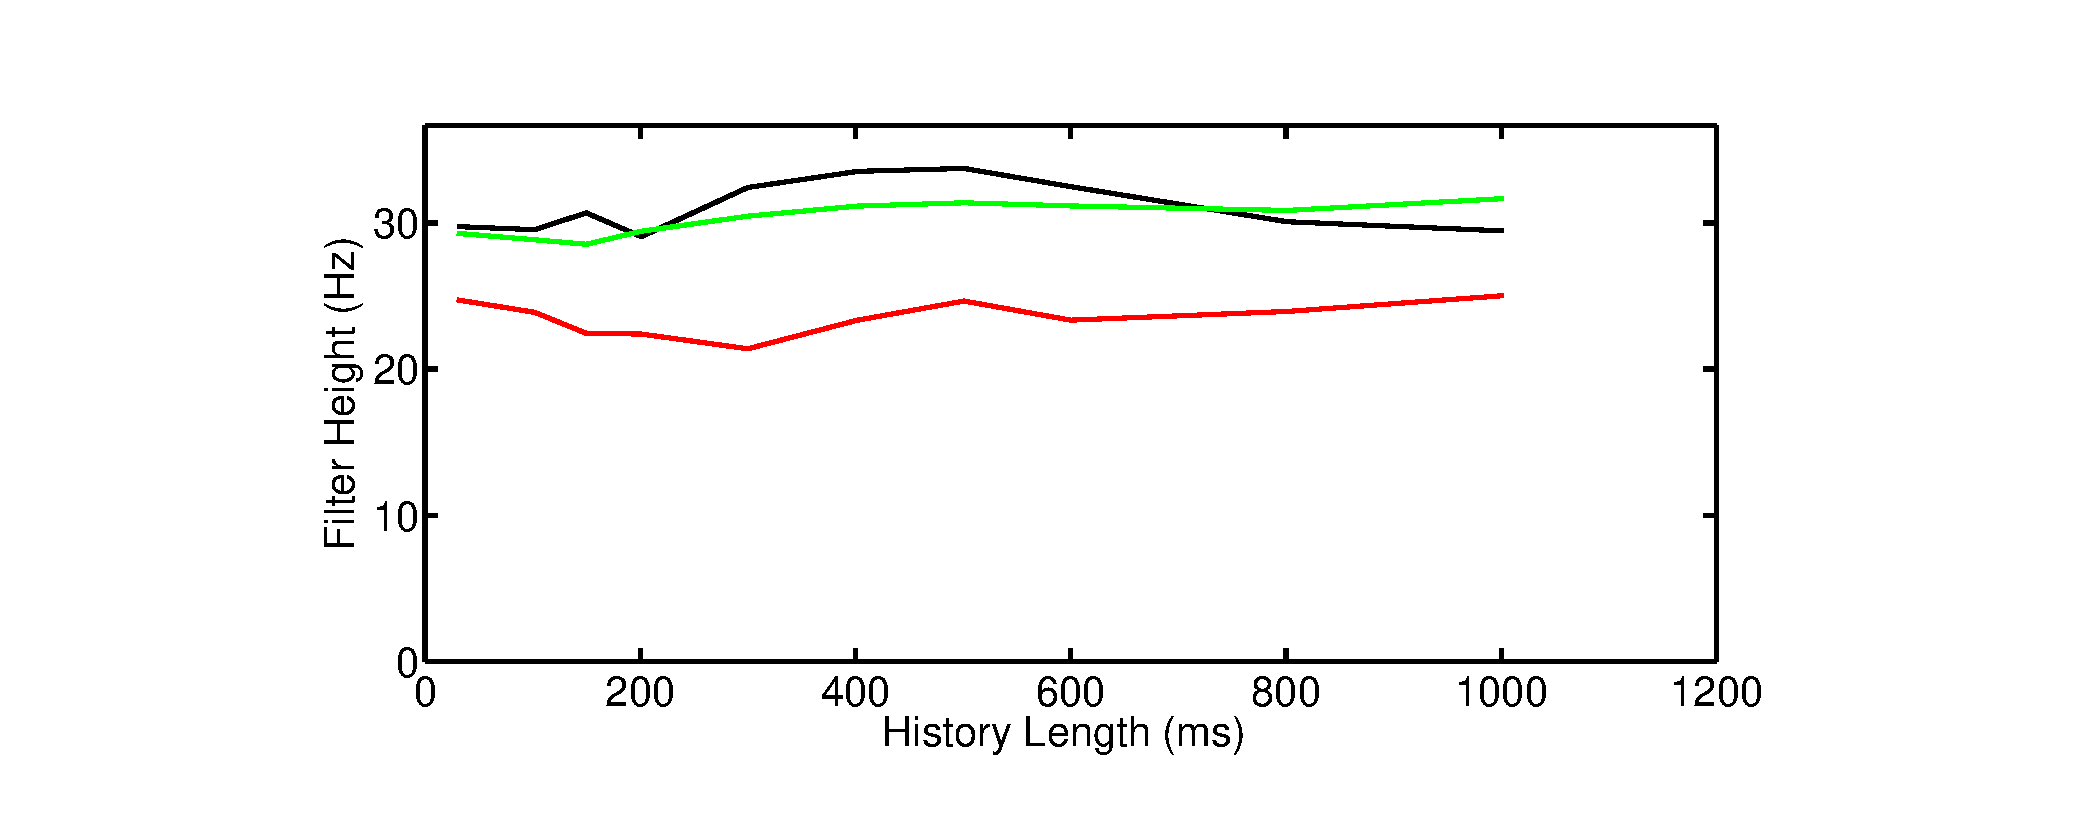
\includegraphics [width=\textwidth]{Analysis_January_11.pdf}
\begin{par}
and use this filter to predict the residuals from the stimulus.
\end{par} \vspace{1em}

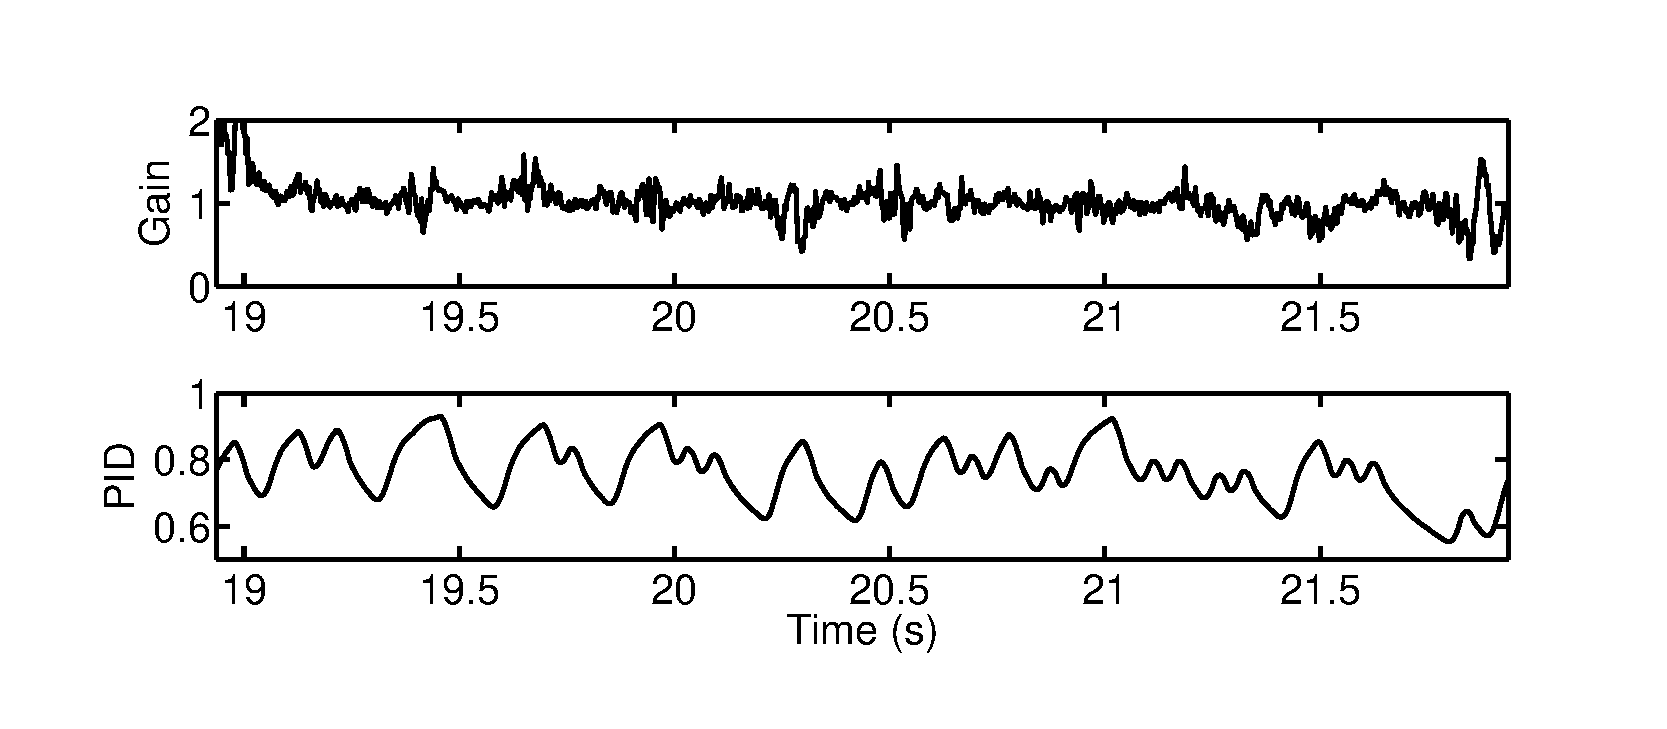
\includegraphics [width=\textwidth]{Analysis_January_12.pdf}
\begin{par}
Does adding this back to the prediction improve the prediction? The following plot shows the data (black), the linear prediction (red), and the linear prediction corrected by the prediciton of the residual (green).
\end{par} \vspace{1em}

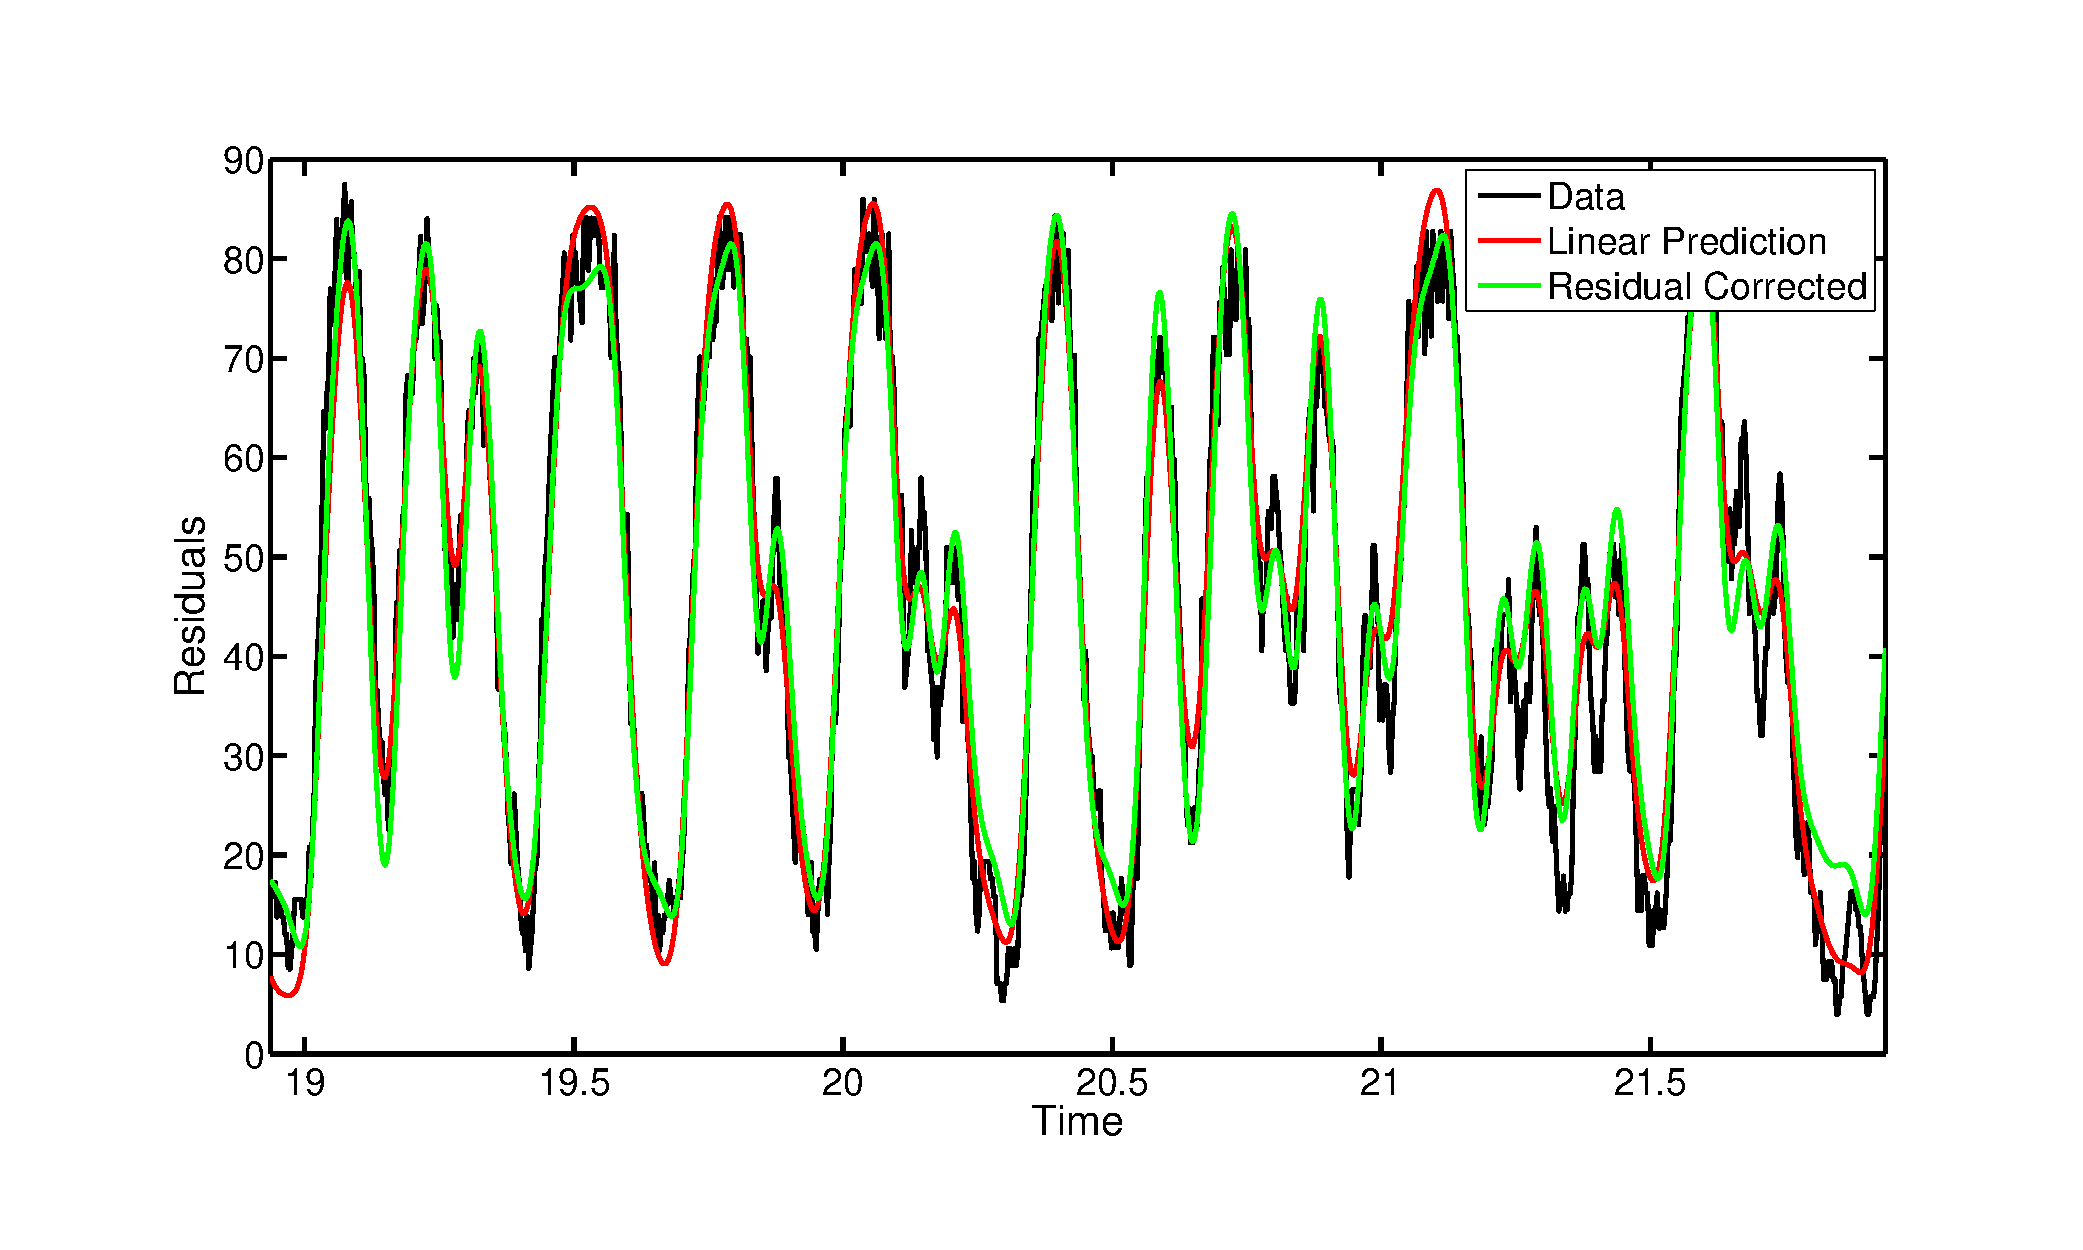
\includegraphics [width=\textwidth]{Analysis_January_13.pdf}
\begin{par}
The r-square of the corrected prediction is
\end{par} \vspace{1em}

        \color{lightgray} \begin{verbatim}    0.9282

\end{verbatim} \color{black}
    \begin{par}
and the r-square of the simple linear prediction is
\end{par} \vspace{1em}

        \color{lightgray} \begin{verbatim}    0.9276

\end{verbatim} \color{black}
    \begin{par}
How does this make any sense? If this is true, then simply adding the filters together will yield a better filter, which we should have computed in the very beginning. The filter, the second filter computed from residuals, and their sum is shown in the panel on the left. On the right is a filter with lower regularisation.
\end{par} \vspace{1em}

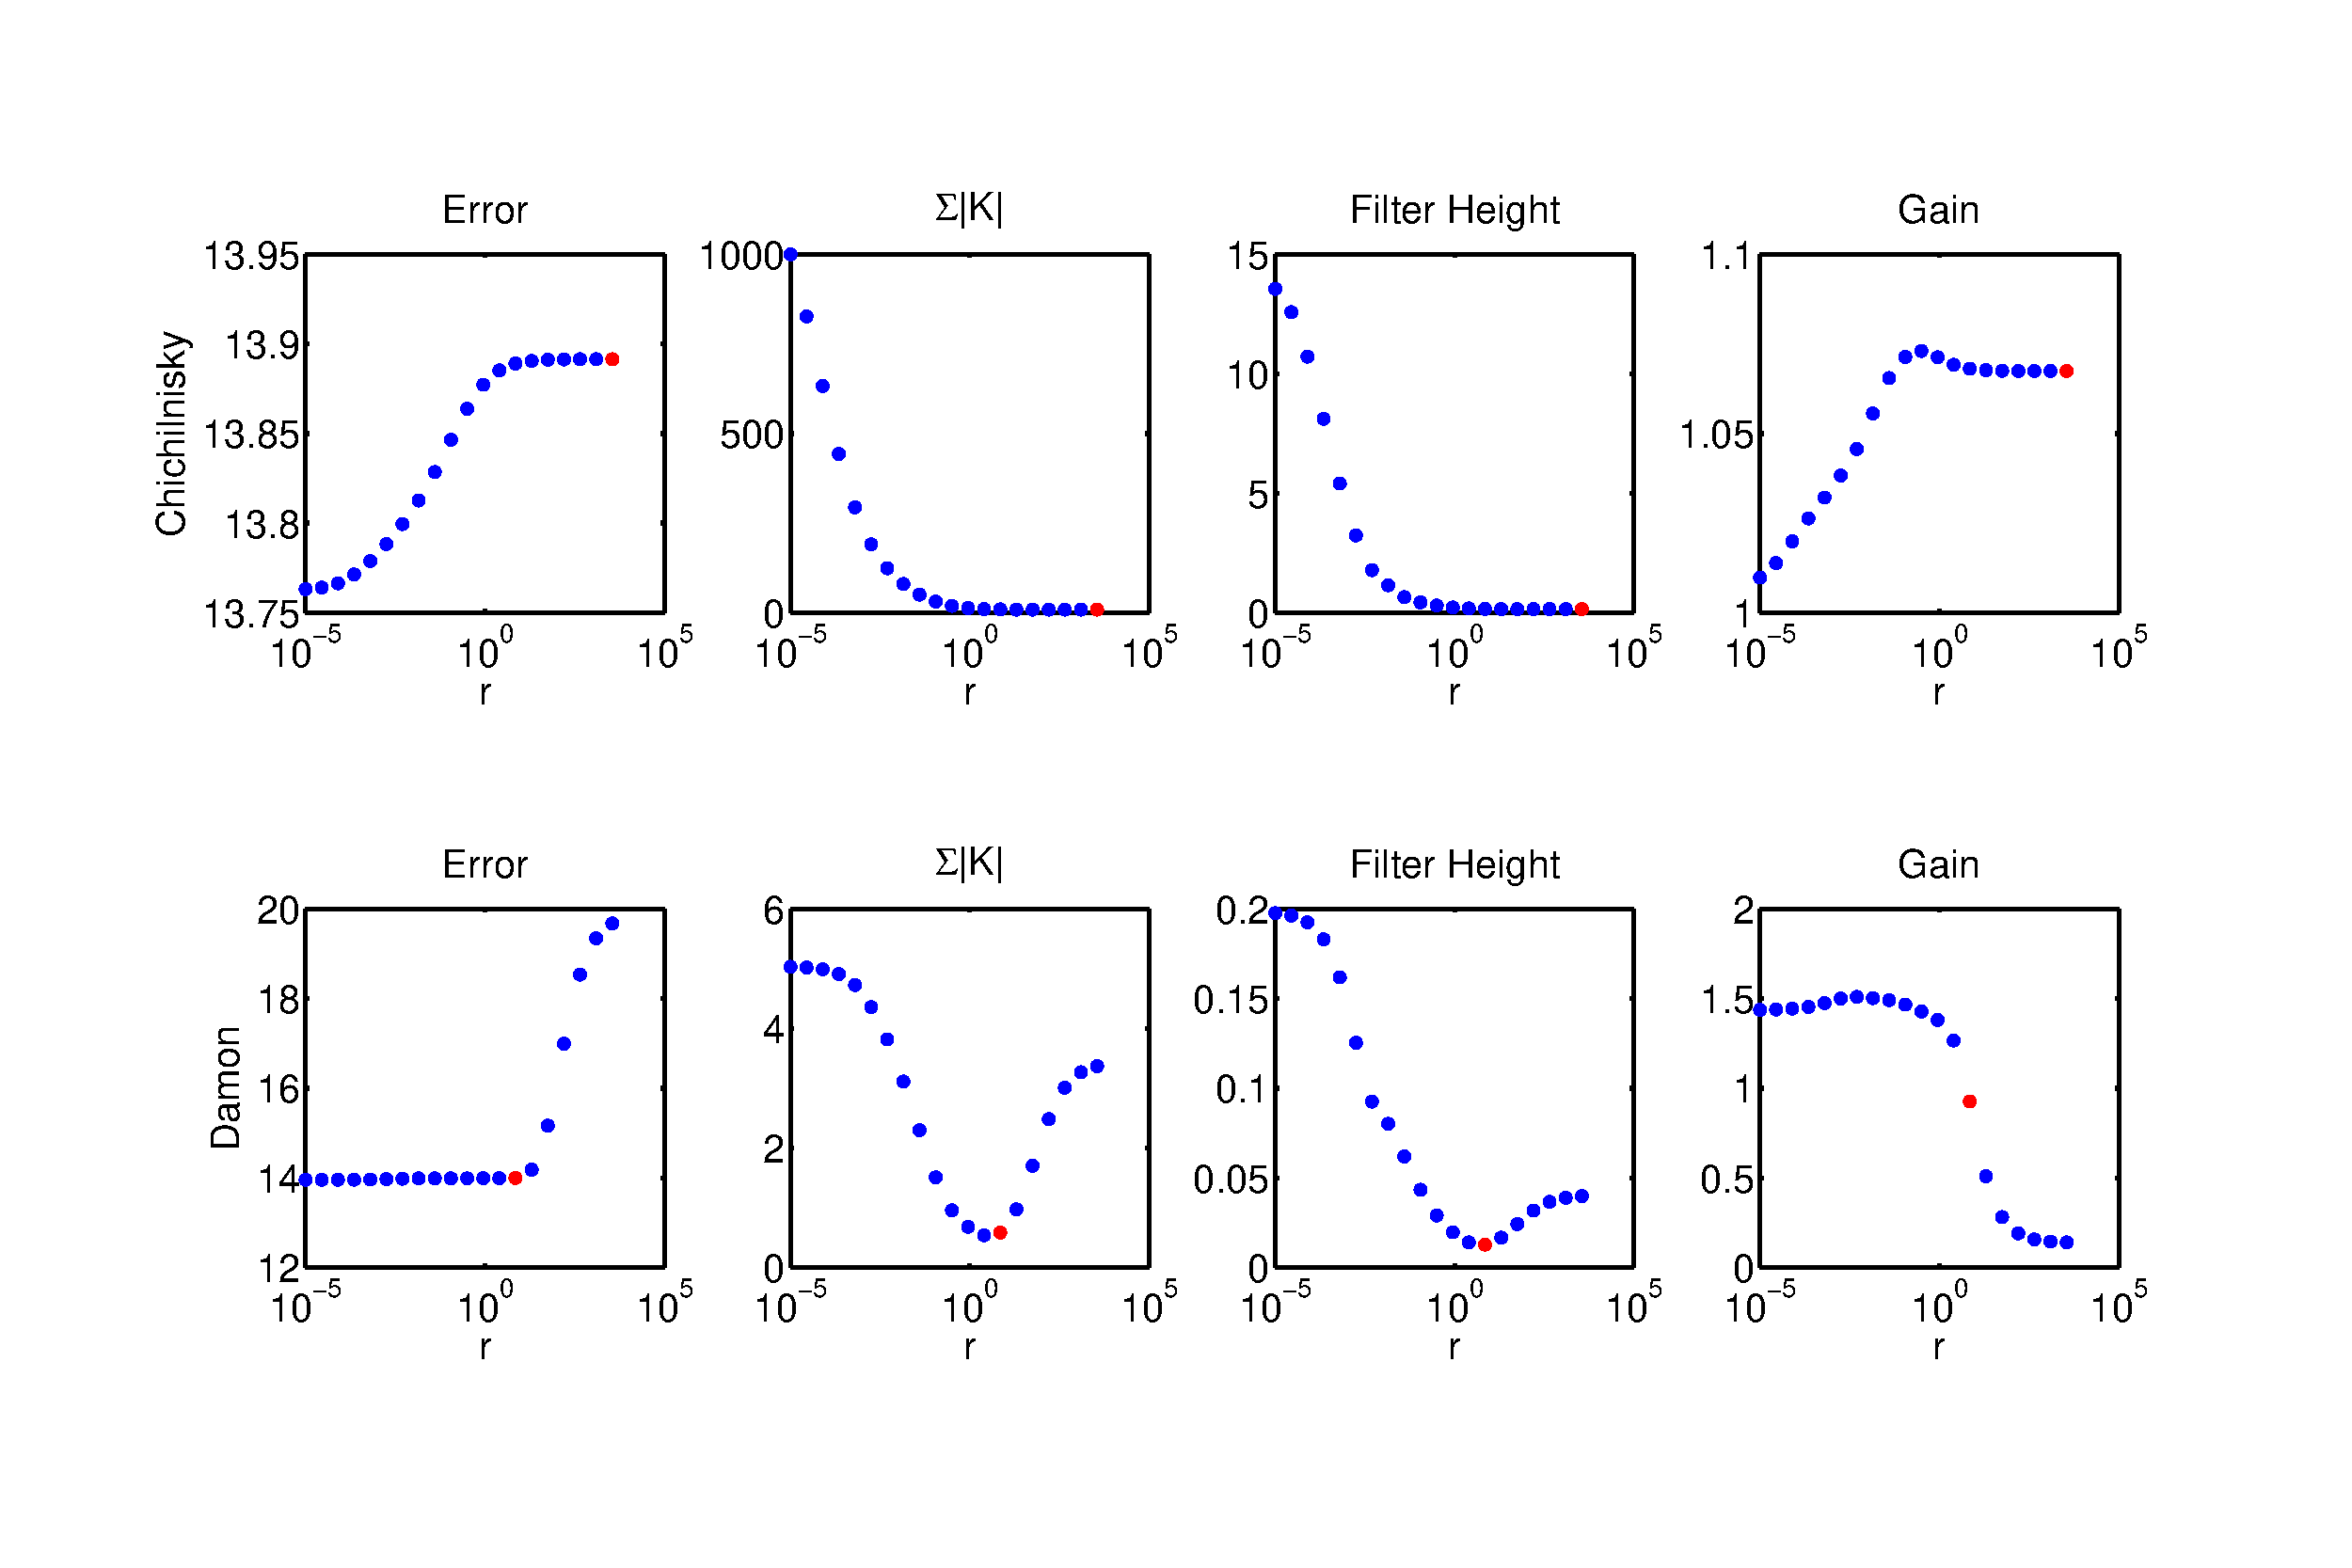
\includegraphics [width=\textwidth]{Analysis_January_14.pdf}
\begin{par}
So what we are doing is simply undoing the work we did in regularising the filter.
\end{par} \vspace{1em}


\subsection*{Analysis of Linear Prediction -  Instantaneous Gain}

\begin{par}
There is a mismatch between the linear prediction and the actual firing rate. Moreover, the instantaneous gain seems to be modulated by something that depends on the past history of the stimulus. Here, in the figure below, the instantaneous gain, i.e., the ratio of the actual firing rate to the predicted firing rate, is plotted along with the stimulus.
\end{par} \vspace{1em}

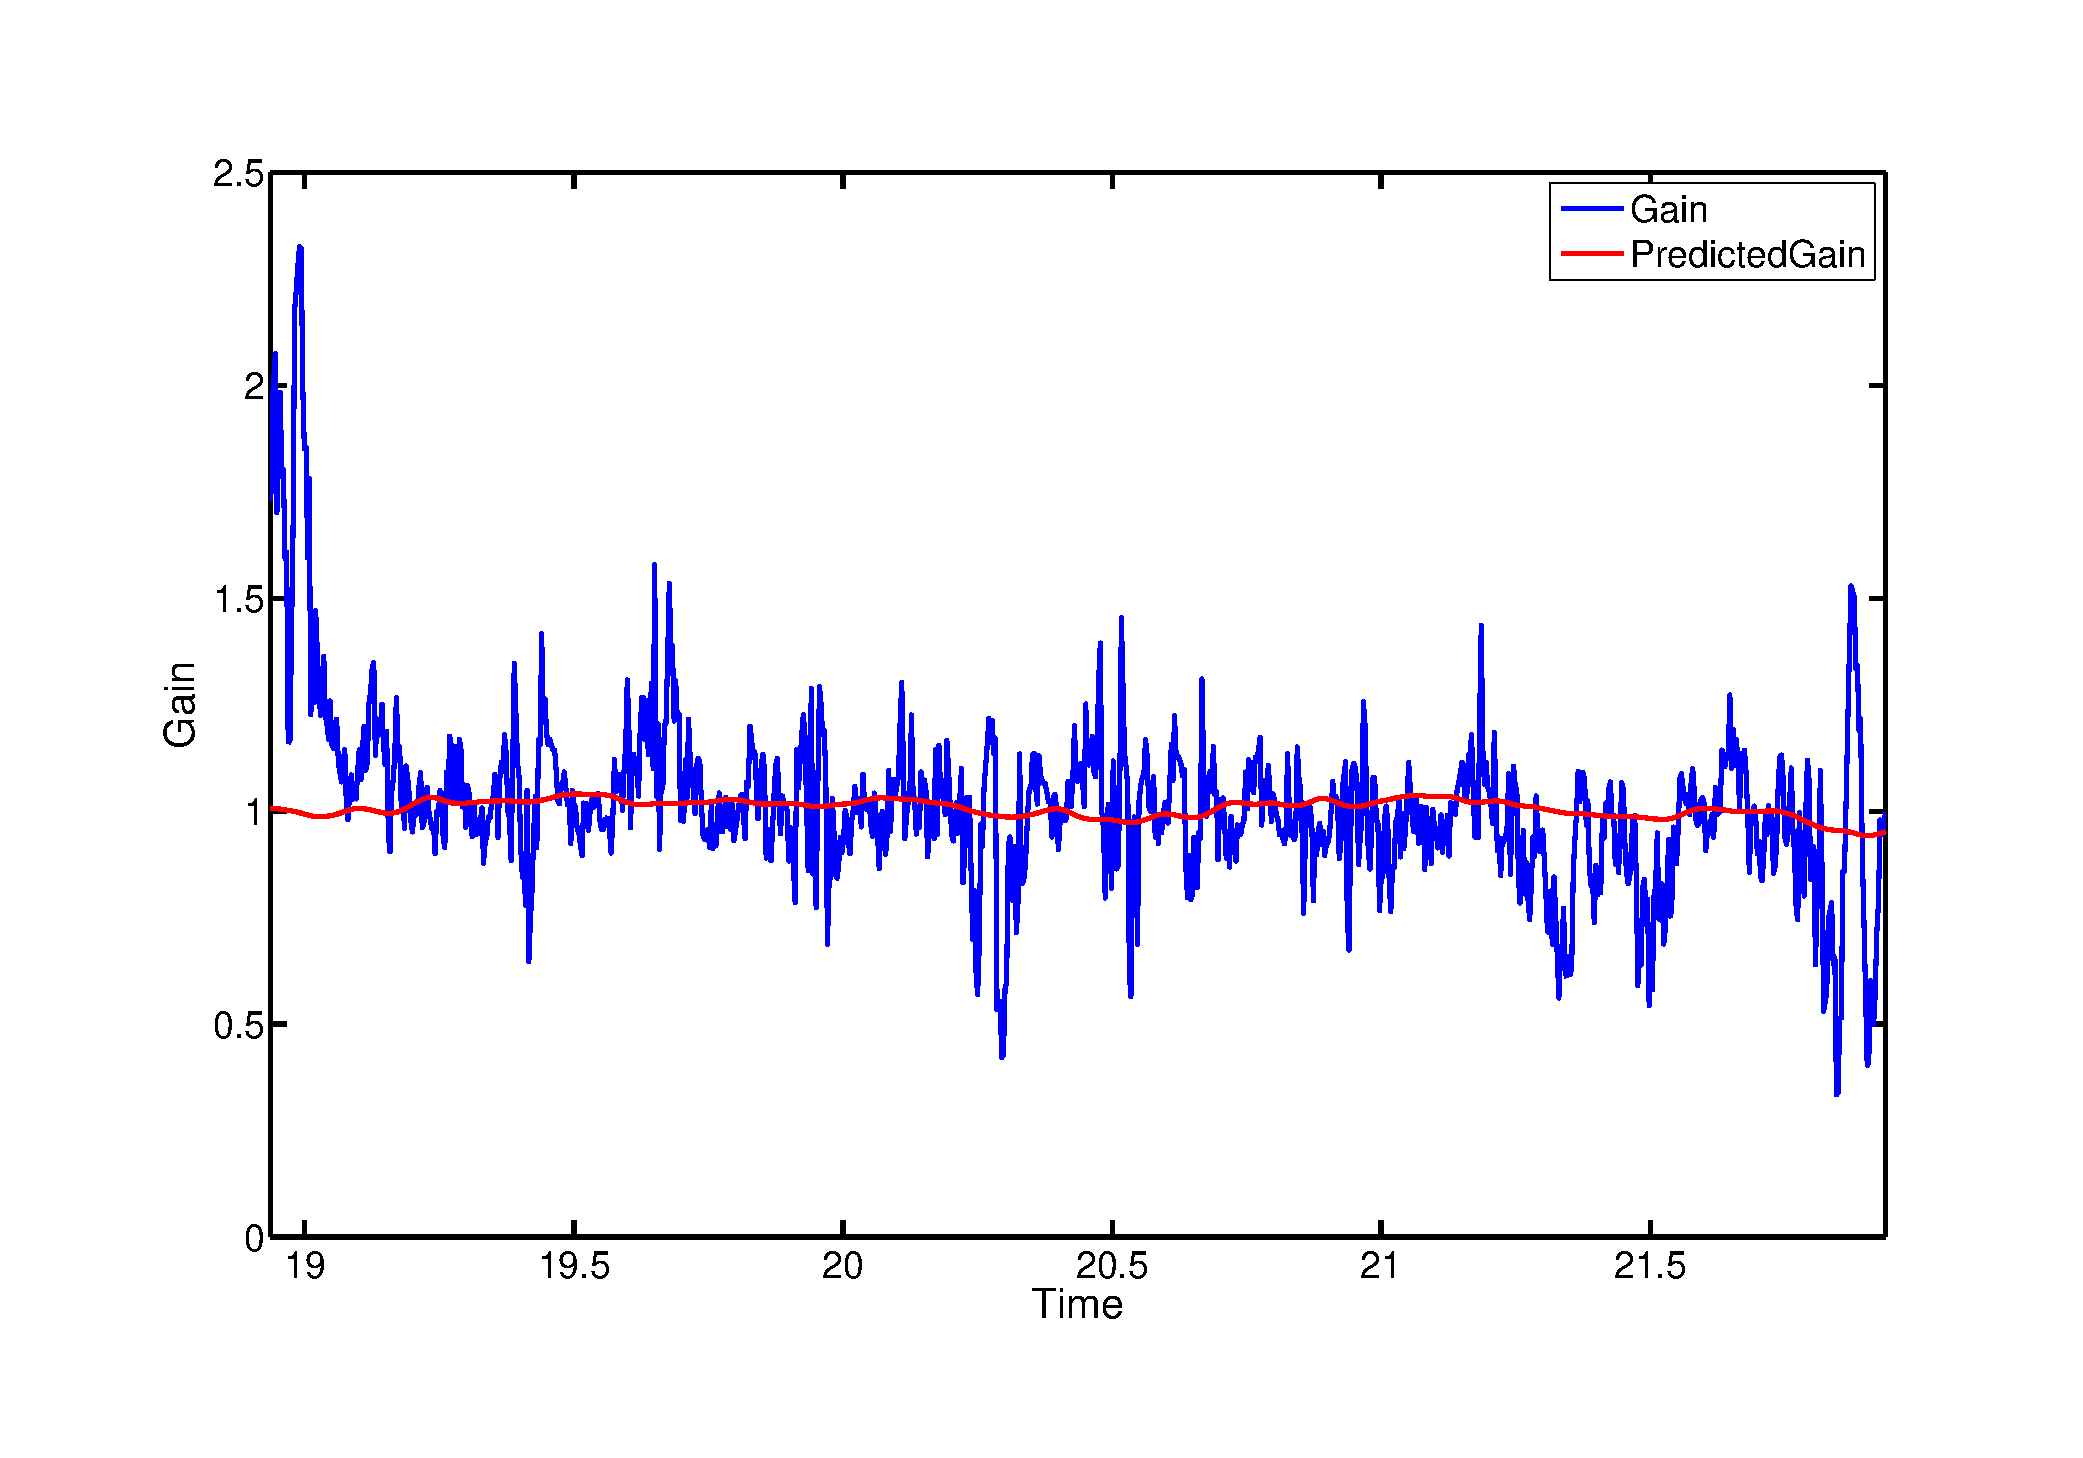
\includegraphics [width=\textwidth]{Analysis_January_15.pdf}
\begin{par}
We can also calculate the moving gain by fitting lines to the data and the prediction collected in bins of size \textit{w}. The following plots show the gain computed in this way for a few different \textit{w}. WARNING. THIS CODE IS SUPER SLOW. FITTING THOUSANDS OF LINES.
\end{par} \vspace{1em}

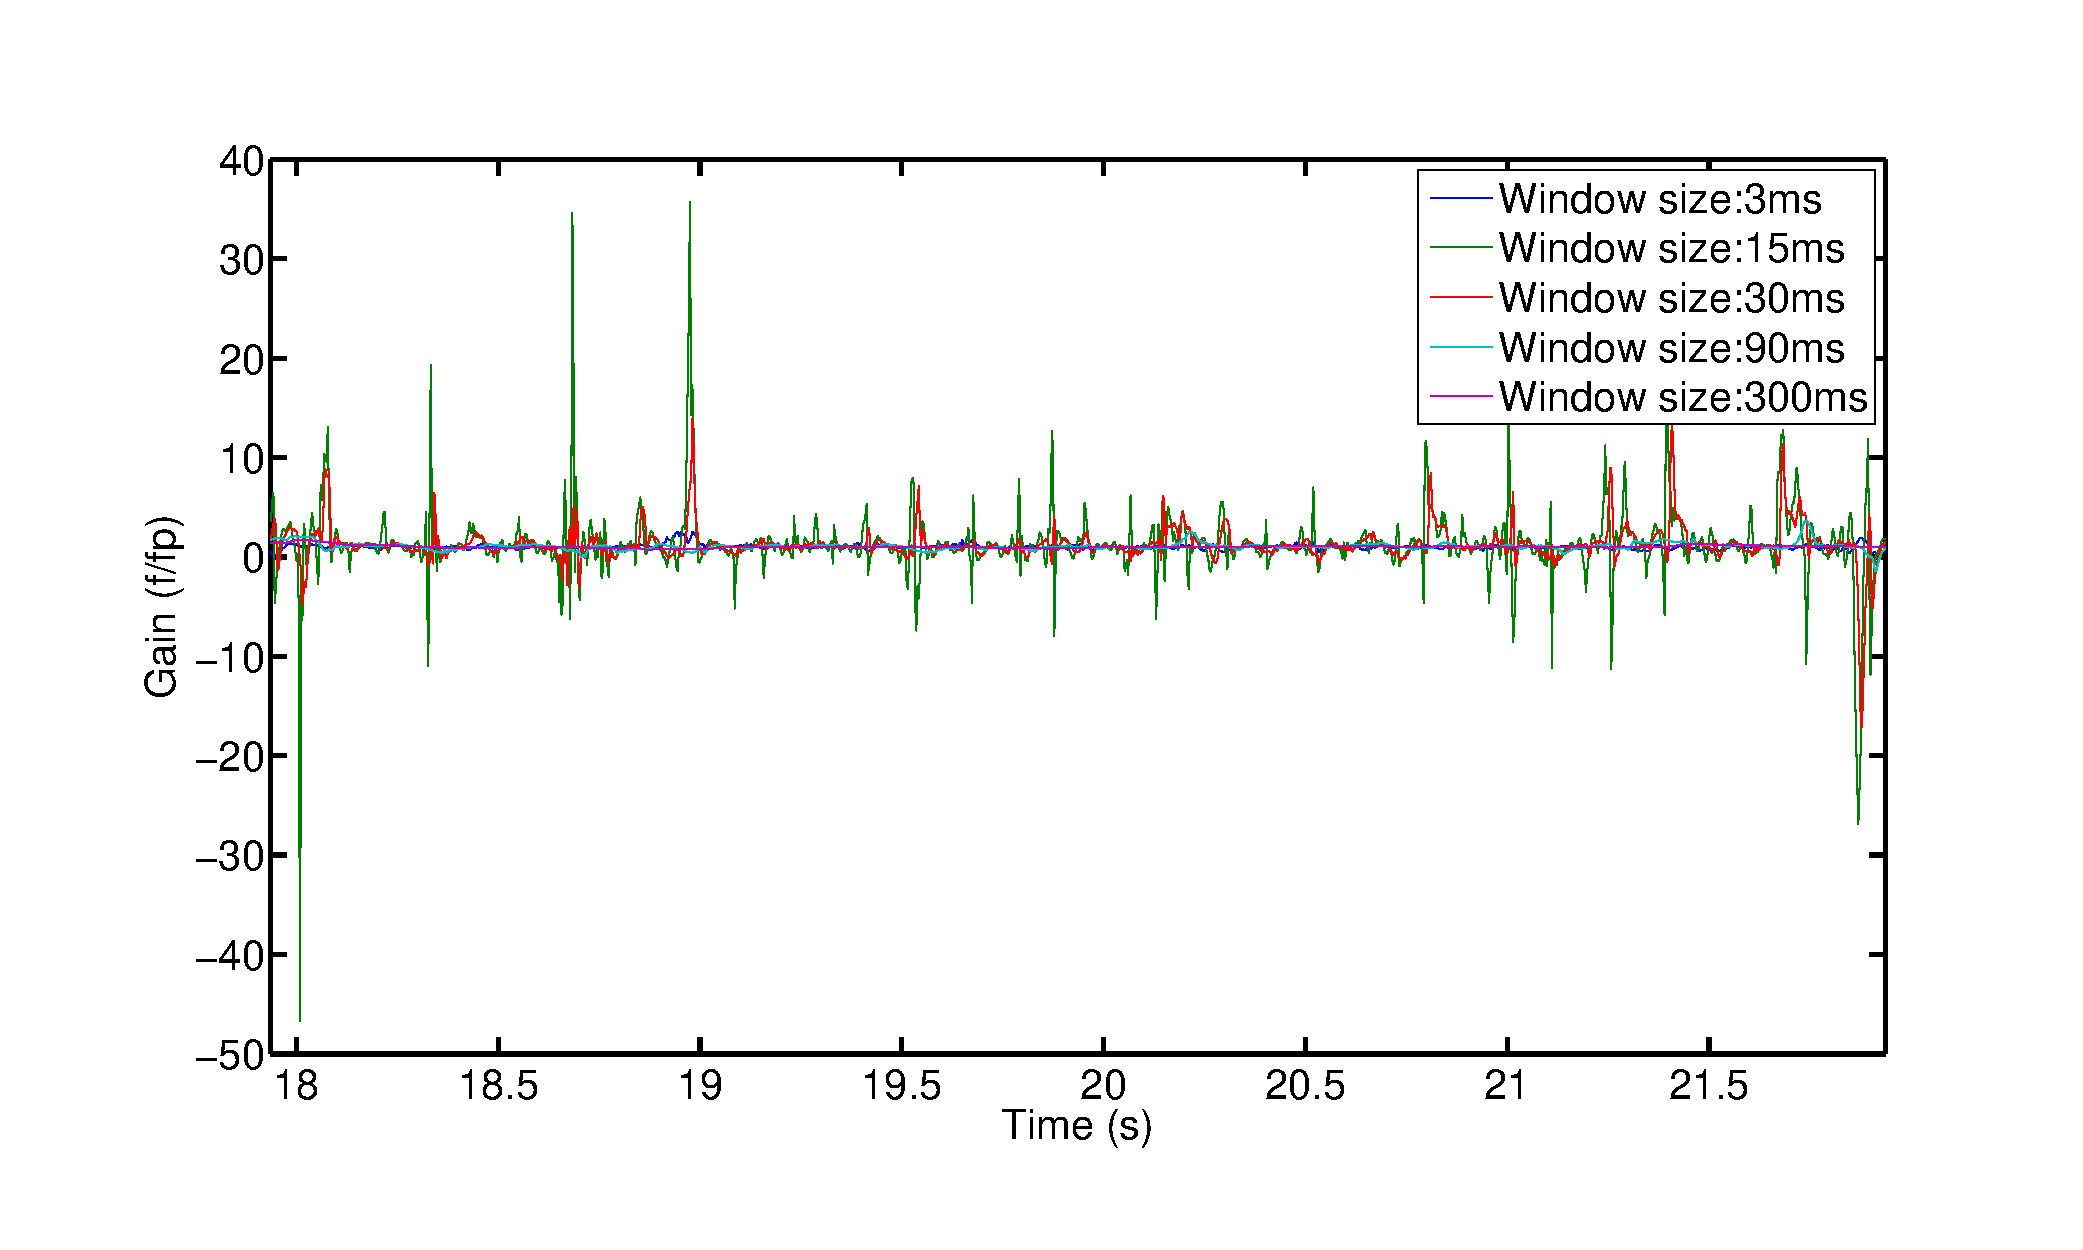
\includegraphics [width=\textwidth]{Analysis_January_16.pdf}
\begin{par}
Of these different gain vectors, which fixes the prediction the best? The following vector is the r-square of prediction, corrected by the each of the gain vectors, scaled by the rsquare of the simple linear prediciton. The first number is \ensuremath{>} 1, indicating that it is an improvement over the simple linear prediction. (In fact, by definition, the first number corresponds to a perfect prediction)
\end{par} \vspace{1em}

        \color{lightgray} \begin{verbatim}    1.0780    0.0007    0.0245    0.4372    0.9184

\end{verbatim} \color{black}
    \begin{par}
Note that none of the scaled r-square values are \ensuremath{>} 1 for any of the fits (points \ensuremath{>} 3ms) so this method of finding the gain is not helpful in improving the prediction.
\end{par} \vspace{1em}
\begin{par}
In the above analysis, we have considered how a boxcar average over the stimulus immediately preceding the current time affects gain. Now, we want to find some optimal way of averaging the past stimulus history to predict the instantaneous gain: by doing so, we can then predict instantaneous gain, and thus get a better predictor of the actual firing rate.
\end{par} \vspace{1em}
\begin{par}
In effect, we can calculate a new filter, $K_g$ such that
\end{par} \vspace{1em}
\begin{par}
$$ K_g=\hat{C}\setminus(s'*g) $$
\end{par} \vspace{1em}
\begin{par}
where \textit{g} is the instantaneous gain (the point-by-point ratio of the data to the linear prediction) and \textit{s} is the stimulus.
\end{par} \vspace{1em}
\begin{par}
Once again, we can look at how filter shape is affected by our choise of \textit{r} for the PID \ensuremath{>} gain prediction:
\end{par} \vspace{1em}
\begin{par}
Once again, we can look at how filter shape is affected by our choise of \textit{r} for the PID \ensuremath{>} gain prediction:
\end{par} \vspace{1em}
\begin{par}
From this filter and the stimulus, we can estimate the instantaneous gain (where the instantaneous gain is defined to be the ratio of the actual firing rate to the linear predicted firing rate)
\end{par} \vspace{1em}
\begin{par}
Using these estimates, we can then correct the linear prediction of the firing rate.
\end{par} \vspace{1em}
\begin{par}
Is the gain-corrected prediction any better than the linear prediction? The r-square of the PID gain corrected estimate is:
\end{par} \vspace{1em}
\begin{par}
The r-square of the Valve gain corrected estimate is:
\end{par} \vspace{1em}
\begin{par}
This is in comparison to the simple linear prediction with a r-square of:
\end{par} \vspace{1em}
\begin{par}
The autocorrelation function of the gain shows that it is very tightly constrained, almost as much as the valve, and much less than the PID, which we are trying to use to predict it.
\end{par} \vspace{1em}


\subsection*{Summary/Problems}

\begin{enumerate}
\setlength{\itemsep}{-1ex}
   \item Best fit line of linear prediction to actual data does not have a slope of 1 for Damon's function. For synthetic data the slope of the line is indeed 1. However, in the real data set, it is not, even with no regularisation.
   \item Prediction of gain from past stimulus is very poor. The correlation coefficient of the prediction with the instantaneous gain is \ensuremath{\tilde{\;}} 0.2. For comparison, the corr. coeff. of the firing rate prediction \ensuremath{>} 0.95.
\end{enumerate}


\subsection*{Next Steps}

\begin{enumerate}
\setlength{\itemsep}{-1ex}
   \item Calculate filters for high and low stimulus zones.
   \item Calculate filters after using elastic net regularisation.
   \item Check if someone has looked at Weber's law in olfaction/ORNs
   \item shuffle data to check validity?
   \item fit Dynamical Adaptation model to data?
\end{enumerate}



\end{document}
    
